\documentclass[a4paper,11pt]{book}
%\documentclass[a4paper,twoside,11pt,titlepage]{book}
\usepackage{listings}
\usepackage[utf8]{inputenc}
\usepackage[spanish]{babel}
\usepackage{csquotes} % Añadir csquotes


\usepackage{commands}

\usepackage{multicol}

%\usepackage[style=list, number=none]{glossary} %
%\usepackage{titlesec}
%\usepackage{pailatino}

\decimalpoint\usepackage{dcolumn}
\newcolumntype{.}{D{.}{\esperiod}{-1}}
\makeatletter
\addto\shorthandsspanish{\let\esperiod\es@period@code}
\makeatother

%\usepackage[chapter]{algorithm}
\RequirePackage{verbatim}
%\RequirePackage[Glenn]{fncychap}
\usepackage{fancyhdr}
\usepackage{graphicx}
\usepackage{afterpage}

\usepackage{longtable}

\usepackage[pdfborder={0 0 0}]{hyperref} %referencia

% ********************************************************************
% Re-usable information
% ********************************************************************

% \documentclass[a4paper,12pt]{article}
\usepackage[utf8]{inputenc}
\usepackage{graphicx}
\usepackage{geometry}
\usepackage{changepage}
\usepackage{fancyhdr}
\usepackage{graphicx}
\usepackage{blindtext}
\usepackage{float} % Añadir este paquete para usar la opción 'H'

%\usepackage{natbib}
\usepackage{url} % Este paquete ayuda a formatear correctamente las URLs
\usepackage[backend=bibtex,style=numeric,url=true]{biblatex}
\addbibresource{bibliografia/bibliografia.bib}




\hypersetup{
pdfauthor = {\myName(g20596044@correo.ugr.es)},
pdftitle = {\myTitle},
pdfsubject = {},
pdfkeywords = {palabra_clave1, palabra_clave2, palabra_clave3},
pdfcreator = {LaTeX con el paquete},
pdfproducer = {pdflatex}
}

%\hyphenation{}

%\usepackage{doxygen/doxygen}
%\usepackage{pdfpages}
\usepackage{url}
\usepackage{colortbl,longtable}
\usepackage[stable]{footmisc}
%\usepackage{index}

\makeindex

%\usepackage[style=long,cols=2,border=plain,toc=true,number=none]{glossaries}
\usepackage{glossaries}
\makeglossaries

% Definición de comandos que me son tiles:
%\renewcommand{\indexname}{Índice alfabético}
%\renewcommand{\glossaryname}{Glosario}

\pagestyle{fancy}
\fancyhf{}
\fancyhead[LO]{\leftmark}
\fancyhead[RE]{\rightmark}
\fancyhead[RO,LE]{\textbf{\thepage}}
\renewcommand{\chaptermark}[1]{\markboth{\textbf{#1}}{}}
\renewcommand{\sectionmark}[1]{\markright{\textbf{\thesection. #1}}}

\setlength{\headheight}{1.5\headheight}

\newcommand{\HRule}{\rule{\linewidth}{0.5mm}}
%Definimos los tipos teorema, ejemplo y definición podremos usar estos tipos
%simplemente poniendo \begin{teorema} \end{teorema} ...
\newtheorem{teorema}{Teorema}[chapter]
\newtheorem{ejemplo}{Ejemplo}[chapter]
\newtheorem{definicion}{Definición}[chapter]

\definecolor{gray97}{gray}{.97}
\definecolor{gray75}{gray}{.75}
\definecolor{gray45}{gray}{.45}
\definecolor{gray30}{gray}{.94}

\lstset{ frame=Ltb,
   framerule=0.5pt,
   aboveskip=0.5cm,
   framextopmargin=3pt,
   framexbottommargin=3pt,
   framexleftmargin=0.1cm,
   framesep=0pt,
   rulesep=.4pt,
   backgroundcolor=\color{gray97},
   rulesepcolor=\color{black},
   %
   stringstyle=\ttfamily,
   showstringspaces = false,
   basicstyle=\scriptsize\ttfamily,
   commentstyle=\color{gray45},
   keywordstyle=\bfseries,
   %
   numbers=left,
   numbersep=6pt,
   numberstyle=\tiny,
   numberfirstline = false,
   breaklines=true,
   }
 
% minimizar fragmentado de listados
\lstnewenvironment{listing}[1][]
   {\lstset{#1}\pagebreak[0]}{\pagebreak[0]}

\lstdefinestyle{CodigoC}
   {
   basicstyle=\scriptsize,
   frame=single,
   language=C,
   numbers=left
   }
\lstdefinestyle{CodigoC++}
   {
   basicstyle=\small,
   frame=single,
   backgroundcolor=\color{gray30},
   language=C++,
   numbers=left
   }

\lstdefinestyle{Consola}
   {basicstyle=\scriptsize\bf\ttfamily,
    backgroundcolor=\color{gray30},
    frame=single,
    numbers=none
   }

\newcommand{\bigrule}{\titlerule[0.5mm]}

%Para conseguir que en las páginas en blanco no ponga cabecerass
\makeatletter
\def\clearpage{%
  \ifvmode
    \ifnum \@dbltopnum =\m@ne
    \ifdim \pagetotal <\topskip
      \hbox{}
    \fi
    \fi
  \fi
  \newpage
  \thispagestyle{empty}
  \write\m@ne{}
  \vbox{}
  \penalty -\@Mi
}
\makeatother

\usepackage{pdfpages}
\begin{document}

% Aquí se incluye la portada del documento
\newgeometry{top=2.3cm, bottom=2.3cm, left=2.3cm, right=2.3cm}
\begin{titlepage}

    \begin{adjustwidth}{4cm}{0cm}

        \begin{flushright}
            \normalsize \myUni| \myDepartment\\[0.1cm]
            \normalsize \myDate\\[4cm]
        \end{flushright}

        \begin{flushleft}   
            {\Huge \textbf{\myTitle}} \\[0.5cm]
            {\Large \mySubTitle} \\[0.5cm]
            \hrulefill \\[0.5cm]
            \textbf{\Large Trabajo de Fin de Grado}\\[3cm]
            
            \textbf{\large \myName} \\[0.1cm]
            \large \textbf{Supervisor}: \myProf\\[2cm]
            
        \end{flushleft}

    \end{adjustwidth}

    \vfill
        \begin{flushleft}
            
\includegraphics[width=0.5\textwidth]{imagenes/logo_2.png}
            \hfill
            
\includegraphics[width=0.15\textwidth]{imagenes/etsiit_logo_3.png}\\[0.5cm]
        \end{flushleft}
\end{titlepage}

   

   





\restoregeometry

% Aquí se incluye el prefacio del documento
\chapter*{}
%\thispagestyle{empty}
%\cleardoublepage

%\thispagestyle{empty}

% No quiero 2 portadas 
%\begin{titlepage}

    \begin{adjustwidth}{4cm}{0cm}

        \begin{flushright}
            \normalsize \myUni| \myDepartment\\[0.1cm]
            \normalsize \myDate\\[4cm]
        \end{flushright}

        \begin{flushleft}   
            {\Huge \textbf{\myTitle}} \\[0.5cm]
            {\Large \mySubTitle} \\[0.5cm]
            \hrulefill \\[0.5cm]
            \textbf{\Large Trabajo de Fin de Grado}\\[3cm]
            
            \textbf{\large \myName} \\[0.1cm]
            \large \textbf{Supervisor}: \myProf\\[2cm]
            
        \end{flushleft}

    \end{adjustwidth}

    \vfill
        \begin{flushleft}
            
\includegraphics[width=0.5\textwidth]{imagenes/logo_2.png}
            \hfill
            
\includegraphics[width=0.15\textwidth]{imagenes/etsiit_logo_3.png}\\[0.5cm]
        \end{flushleft}
\end{titlepage}

   

   






%\cleardoublepage
%\thispagestyle{empty}

\begin{center}
{\large\bfseries \myTitle: \mySubTitle}\\
\end{center}
\begin{center}
\myName\\
\end{center}

% Palabras Clave
%\vspace{0.7cm}
\noindent{\textbf{Palabras clave}:}
\begin{itemize}
       \item \textbf{HPC}: También conocida como supercomputación, es un área de la informática en la que el rendimiento es el principal criterio de optimización, enfocándose en la capacidad de procesar grandes volúmenes de datos y realizar cálculos complejos

\end{itemize}

\vspace{0.7cm}
\noindent{\textbf{Resumen}}\\


En este proyecto se propone la implementación y evaluación de un servidor HPC (High Performance Computing), con un enfoque principal en comprender y documentar su ciclo de vida completo, desde el montaje inicial hasta su utilización. Esto representa mis primeros pasos consolidados en el ámbito del mantenimiento y despliegue de servidores, una tarea para la cual la experiencia en unas prácticas Erasmus como IT Infrastructure en Alemania, centrada en el montaje y despliegue de servidores, proporciona una base sólida.

Una vez configurado y operativo el servidor HPC, se procederá con una estrategia dual para evaluar su rendimiento y utilidad. En primer lugar, se realizará el despliegue de modelos de lenguaje (LLM) de gran escala y varios modelos pequeños utilizando contenedores con acceso a unidades de procesamiento gráfico (GPU). Se llevarán a cabo benchmarks comparativos para evaluar su rendimiento y eficiencia, demostrando así la capacidad de la infraestructura HPC establecida.

En segundo lugar, y aprovechando la infraestructura montada, se implementará un entorno de orquestación local. Este entorno simulará un ecosistema de producción con el fin de demostrar y validar los principios fundamentales de Site Reliability Engineering (SRE). Finalmente, se utilizará la plataforma de orquestación para examinar y validar capacidades avanzadas de SRE, tales como el escalado automático de recursos, la recuperación autónoma ante fallos y los procedimientos de despliegue continuo (CI/CD) desde repositorios de control de versiones.

\cleardoublepage


\thispagestyle{empty}


\begin{center}
{\large\bfseries \myTitleE: \mySubTitleE}\\
\end{center}
\begin{center}
\myName\\
\end{center}

%\vspace{0.7cm}
\noindent{\textbf{Keywords}: Keyword1, Keyword2, Keyword3, ....}\\

\vspace{0.7cm}
\noindent{\textbf{Abstract}}\\

This project proposes the implementation and evaluation of a High Performance Computing (HPC) server. The primary focus is to thoroughly understand and document its complete lifecycle, from initial assembly to its full utilization. This endeavor represents my first consolidated steps in server maintenance and deployment, an area where my Erasmus internship experience as IT Infrastructure in Germany, centered on server assembly and deployment, provides a solid foundation.

Once the HPC server is configured and operational, a dual strategy will be employed to assess its performance and utility. Firstly, we will deploy large-scale Language Models (LLMs) and several smaller models using containers with access to Graphics Processing Units (GPUs). Comparative benchmarks will be conducted to evaluate their performance and efficiency, thereby demonstrating the capabilities of the established HPC infrastructure.

Secondly, leveraging the assembled infrastructure, a local orchestration environment will be implemented. This environment will simulate a production ecosystem to demonstrate and validate the fundamental principles of Site Reliability Engineering (SRE). Finally, the orchestration platform will be used to examine and validate advanced SRE capabilities, such as automatic resource scaling, autonomous fault recovery, and continuous integration/continuous deployment (CI/CD) procedures from version control repositories.


\chapter*{}
\thispagestyle{empty}

\noindent\rule[-1ex]{\textwidth}{2pt}\\[4.5ex]

Yo, \textbf{\myName}, alumno de la titulación \myDegree de la \textbf{Escuela Técnica Superior
de Ingenierías Informática y de Telecomunicación de la Universidad de Granada}, con DNI 20596044G, autorizo la
ubicación de la siguiente copia de mi Trabajo Fin de Grado en la biblioteca del centro para que pueda ser
consultada por las personas que lo deseen.

\vspace{6cm}

\noindent Fdo: \myName

\vspace{2cm}

\begin{flushright}
\myDate
\end{flushright}


\chapter*{}
\thispagestyle{empty}

\noindent\rule[-1ex]{\textwidth}{2pt}\\[4.5ex]

D. \textbf{\myProf}, Profesor del Área de Ingeniería Informática del \myDepartment\\ de la Universidad de Granada.

\vspace{0.5cm}

% D. \textbf{Nombre Apellido1 Apellido2 (tutor2)}, Profesor del Área de XXXX del Departamento YYYY de la Universidad de Granada.

% \vspace{0.5cm}

\textbf{Informan:}

\vspace{0.5cm}

Que el presente trabajo, titulado \textit{\textbf{\myTitle, \mySubTitle}},
ha sido realizado bajo su supervisión por \textbf{\myName}, y autorizamos la defensa de dicho trabajo ante el tribunal
que corresponda.

\vspace{0.5cm}

Y para que conste, expiden y firman el presente informe en \myDate\\.

\vspace{1cm}

\textbf{Los directores:}

\vspace{5cm}

%\noindent \textbf{Nombre Apellido1 Apellido2 (tutor1) \ \ \ \ \ Nombre Apellido1 Apellido2 (tutor2)}

\noindent \textbf{\myProf}


\chapter*{Agradecimientos}
\thispagestyle{empty}

       \vspace{1cm}


Dedicado a mi familia, que siempre me han apoyado en mis decisiones y me han hecho ser quien soy hoy. A mis amigos, que siempre han estado ahí para ayudarme y apoyarme en los momentos difíciles.  Y a todos los profesores y compañeros de la Universidad de Granada, que me han dado la oportunidad de crecer como persona y profesional.


\frontmatter

% Aquí se genera la tabla de contenidos
\tableofcontents

% Aquí se genera la lista de figuras
\listoffigures

% Aquí se genera la lista de tablas
\listoftables

\mainmatter\setlength{\parskip}{5pt}

% Aquí se incluye el capítulo de introducción
   
\chapter{Introducción}
Este es el contenido del primer capítulo.

% Aquí se pueden incluir otros capítulos comentados
%\input{capitulos/02_EspecificacionRequisitos}
%\input{capitulos/03_Planificacion}
%\input{capitulos/04_Analisis}
%\input{capitulos/05_Diseno}
%\input{capitulos/06_Implementacion}
%\input{capitulos/07_Pruebas}
%\input{capitulos/08_Conclusiones}

\newpage % deja una cara en blanco porque book siempre dice que que los chapters comiencen en paginas impares

\begin{multicols*}{2}
    \chapter{Estado del Arte}
    
    \section{Introducción}
    La computación de alto rendimiento (HPC) es fundamental para la ejecución de cargas de trabajo intensivas, como el despliegue de modelos de inteligencia artificial (IA). En este contexto, los Modelos de Lenguaje Grandes (LLMs) representan un desafío técnico debido a su alta demanda de recursos computacionales y de memoria. Este trabajo se centra en la instalación y configuración de un servidor de alto rendimiento, siendo uno de los objetivos de alojar un LLM utilizando una plataforma de orquestación de contenedores, y en comparar cuantitativamente dos estrategias de despliegue:
    \begin{itemize}
        \item Un único modelo de gran tamaño que atiende múltiples solicitudes.
        \item Múltiples modelos más pequeños especializados en tareas específicas.
    \end{itemize}
    El análisis se basará en métricas como tokens por segundo, uso de recursos (GPU/CPU y memoria) y latencia, entre otras. Para ello, se emplearán benchmarks y herramientas de Site Reliability Engineering (SRE) que garanticen la fiabilidad y resiliencia del sistema.
    
    Toda la documentación de este trabajo se ha gestionado mediante la plataforma Notion, donde se mantiene una bitácora detallada de la planificación del TFG. Del mismo modo, todos los borradores y avances se encuentran organizados en dicho entorno y han sido compartidos con el tutor del proyecto. Se proporcionará un enlace de acceso para su consulta.
    
    \section{Marco Conceptual}
    Con el propósito de contextualizar esta investigación, es necesario definir los conceptos clave que ayudan a comprender mejor la memoria. Además, se incluye un glosario con los términos técnicos relevantes para facilitar la comprensión del lector.
    \begin{itemize}
        \item Infraestructura HPC: Se refiere a una infraestructura computacional diseñada para proporcionar un rendimiento superior en el procesamiento de datos complejos y tareas intensivas desde el punto de vista computacional.
        \item Virtualización: Técnica que, mediante plataformas de orquestación, permite gestionar de forma eficiente los recursos del servidor y coordinar contenedores de manera optimizada.
        \item Benchmarks: Herramientas de evaluación que miden el rendimiento del sistema bajo diferentes configuraciones, proporcionando métricas objetivas para su análisis y optimización.
        \item Site Reliability Engineering (SRE): Disciplina que garantiza la fiabilidad, disponibilidad y rendimiento de los sistemas mediante la aplicación de principios de ingeniería de software a las operaciones.
        \item Modelos de Lenguaje Grandes (LLMs): Sistemas de inteligencia artificial entrenados con grandes cantidades de datos para entender, generar y procesar lenguaje natural.
        \item Tokens por segundo: Métrica que mide la cantidad de tokens (unidades de texto) que un modelo de lenguaje puede procesar o generar en un segundo, indicando su velocidad de inferencia.
    \end{itemize}
    
    \section{Planteamiento del Problema}
    Configurar un servidor de alto rendimiento para desplegar modelos de lenguaje de gran tamaño obliga a resolver tanto retos de rendimiento como de fiabilidad operativa. Para abordarlos se ha diseñado una estrategia en dos partes:
    
    \subsection*{Despliegue y comparativa de varios LLMs}
    Se ejecutará un modelo de gran tamaño por un lado, y se comparará con varios modelos más pequeños dentro de contenedores que utilizan de forma nativa los recursos gráficos del servidor. Este entorno permitirá medir con precisión el consumo de VRAM, la ocupación de memoria y la velocidad de inferencia, sin la sobrecarga que introduce la virtualización.
    
    \subsection*{Demostración de prácticas SRE con OpenShift Local}
    De manera complementaria, se habilitará una simulación de un ecosistema de producción, para validar capacidades propias del Site Reliability Engineering: despliegue continuo de servicios a partir de repositorios, escalado automático ante picos de carga, auto-healing tras fallos inducidos y observabilidad integral. Este entorno reproducible facilitará la evaluación de la fiabilidad y de la automatización en producción.
    
    A partir de esta doble aproximación emergen cinco desafíos principales:
    \begin{itemize}
        \item Estrategia de despliegue: Un único modelo grande puede saturar GPU y memoria; varios modelos pequeños añaden complejidad de orquestación y sincronización.
        \item Integración de contenedores en HPC: Adaptar un entorno pensado para cargas monolíticas a una ejecución contenerizada requiere ajustes en red, almacenamiento y seguridad.
        \item Aplicación de prácticas SRE: Introducir monitorización, escalado y recuperación automática en un sistema crítico de inferencia continua es clave para garantizar su disponibilidad.
        \item Benchmarks cuantitativos: Escasean estudios que comparen tokens por segundo, latencia o uso de caché entre distintas estrategias de despliegue en entornos de alto rendimiento.
        \item Aprendizaje operativo: Administrar un servidor de esta envergadura exige adquirir destrezas en instalación física, configuración de hardware y resolución de incidencias; documentar ese proceso resulta esencial para transferir el conocimiento.
    \end{itemize}
    
    \section{Pregunta de Investigación}
    \textit{¿Qué diferencias de rendimiento y eficiencia aparecen al desplegar un único modelo de lenguaje de gran tamaño frente a varios modelos más pequeños en un servidor HPC, y de qué manera las prácticas de Site Reliability Engineering pueden complementar esa estrategia para asegurar su fiabilidad y mantenimiento a largo plazo?}

    Para abordar esta pregunta de investigación, se adoptará un enfoque de “Divide y Vencerás”, descomponiendo el problema en las siguientes dimensiones críticas:
    
    \subsection*{Rendimiento y eficiencia en el uso de recursos}
    \textit{¿Cómo afecta la elección entre un único modelo grande y múltiples modelos pequeños al rendimiento y la eficiencia en el uso de recursos del servidor HPC, incluyendo el uso de GPUs, memoria RAM y ancho de banda de red?}
    Esta dimensión busca cuantificar el impacto sobre el rendimiento del hardware y la optimización de recursos, considerando métricas como la utilización de CPU/GPU y la eficiencia energética.
    
    \subsection*{Capacidad de respuesta y escalabilidad}
    \textit{¿Qué enfoque ofrece una mejor capacidad de respuesta (latencia) y escalabilidad frente a un aumento en el número de solicitudes concurrentes, especialmente en un entorno orquestado?}
    Se evaluará cómo cada estrategia maneja la carga de trabajo en escenarios de alta demanda, atendiendo a métricas como tokens por segundo, tiempo de respuesta y capacidad de escalado horizontal.
    
    \subsection*{Aplicación de prácticas SRE para la gestión del despliegue}
    \textit{¿Qué herramientas y prácticas de Site Reliability Engineering (SRE) pueden implementarse para garantizar la fiabilidad, observabilidad y mantenibilidad del despliegue de un LLM en una infraestructura HPC?}
    Se centra en la aplicación de metodologías SRE para mejorar la observabilidad, la gestión de incidentes y la automatización de tareas.
    
    \subsection*{Optimización de tokens por segundo y eficiencia en inferencia}
    \textit{¿Cuál de las dos estrategias permite una mayor generación de tokens por segundo y una mayor eficiencia en la inferencia, considerando la distribución de la carga y la capacidad de procesamiento en un entorno HPC?}
    Se analiza la métrica clave de rendimiento para los modelos de lenguaje, evaluando la velocidad de generación de tokens y la eficiencia en la ejecución de tareas de inferencia. Este análisis proporciona un punto de partida sólido para comprender el comportamiento de los modelos en entornos de alto rendimiento.


    \section{Metodología de Revisión y Búsqueda de Información}
Para profundizar en este estudio, es fundamental realizar una revisión del estado del arte, lo que permitirá identificar las bases teóricas en las que se sustenta este trabajo. Esta fase de revisión tiene como objetivo principal detectar carencias en áreas como los despliegues en entornos HPC, la implementación de modelos de lenguaje (LLMs) y el uso de prácticas de Site Reliability Engineering (SRE). Al identificar aspectos que aún no han sido suficientemente explorados, es posible orientar el proyecto hacia líneas de investigación con mayor impacto, sentando así las bases para una propuesta sólida e innovadora.

Para llevar a cabo esta revisión, se comenzará identificando las palabras clave y los términos relacionados con los conceptos centrales del proyecto. Estas palabras clave facilitarán la búsqueda de fuentes de calidad, asegurando que la información recopilada sea precisa, pertinente y útil para el desarrollo de la investigación.

\subsection*{Términos principales}
\begin{itemize}
    \item "Site Reliability Engineering", "SRE"
    \item "High Performance Computing", "HPC"
    \item "GPU server", "Machine Learning infrastructure", "MLOps"
    \item "Virtualization", "Containerization", "Orchestration"
    \item "OpenShift", "Kubernetes"
    \item "Service Level Objectives", "SLOs", "Service Level Indicators", "SLIs"
    \item "Reliability", "Scalability", "Security", "Automation", "Monitoring"
\end{itemize}

\subsection*{Términos relacionados y sinónimos}
\begin{itemize}
    \item Para \textit{Reliability}: \textit{Fault Tolerance}, \textit{Availability}, \textit{Resilience}
    \item Para \textit{Performance}: \textit{Throughput}, \textit{Latency}, \textit{Efficiency}
    \item Para \textit{Deployment}: \textit{Scaling}, \textit{Resource Allocation}, \textit{Load Balancing}
\end{itemize}

\subsection*{Referencias Bibliográficas Clave}
La búsqueda de información se centrará en fuentes académicas reconocidas, tales como \textit{IEEE Xplore}, \textit{ACM Digital Library}, \textit{arXiv} o \textit{Google Scholar} entre otros, así como en la colección digital de la universidad como \textit{O'Reilly} y recursos técnicos oficiales relevantes. Para facilitar el proceso, se emplea \textit{Elicit}, una herramienta basada en inteligencia artificial, con el fin de agilizar la búsqueda dentro de los repositorios mencionados, mapear referencias relacionadas y sintetizar información relevante.

Por otra parte, se dará preferencia a trabajos que aborden la implementación de Site Reliability Engineering (SRE) en entornos HPC, la gestión de infraestructura basada en GPU para aplicaciones de inteligencia artificial, así como estudios sobre métricas de servicio y automatización. Se descartaron fuentes no académicas o desactualizadas.

La información recopilada será organizada en la plataforma Notion, registrando detalles como autoría, año de publicación y una justificación de su relevancia. Posteriormente, será analizada críticamente con el objetivo de identificar tanto las principales contribuciones como las lagunas existentes en la literatura. Se incluye a continuación el enlace a la tabla resultante.

% poner la tabla aqui 

\section{Análisis Comparativo de Herramientas de Orquestación}
Una vez establecida la base teórica y documental, se va a debatir cuál es la herramienta que vamos a utilizar para orquestar los servicios necesarios para nuestro proyecto de investigación. Para ello, se van a comparar cuatro herramientas de orquestación muy conocidas y utilizadas en la industria: Kubernetes, Docker Swarm, OpenShift y Apache Mesos. La razón por la que seleccionamos estas herramientas es que son las más conocidas y confiables en la industria, están probadas en entornos de producción y tienen la capacidad de trabajar sin problemas en infraestructuras de alto rendimiento, como los servidores HPC.
Estas herramientas se analizan a partir de cinco criterios fundamentales:
\begin{itemize}
    \item Desarrollo activo
    \item Facilidad de uso
    \item Flexibilidad para entornos diversos
    \item Rendimiento óptimo
    \item Integración con prácticas de Site Reliability Engineering (SRE)
\end{itemize}

\subsection*{Kubernetes}
Kubernetes, lanzado por Google en 2015, es actualmente la plataforma de orquestación más adoptada, con una cuota de mercado del 77\% (2020) \cite{arxiv_2211_07032} y el respaldo de una comunidad activa internacional. En cuanto a la adaptabilidad, Kubernetes puede desplegarse en "casi cualquier plataforma", lo que lo convierte en una opción altamente versátil. Respecto al rendimiento, destaca por sus "mejores características de programación" (scheduling features), esenciales para optimizar cargas de trabajo en entornos HPC. Kubernetes ofrece funcionalidades como "self-healing", escalabilidad y gestión del ciclo de vida de contenedores, aspectos clave para garantizar la fiabilidad y resiliencia de los servicios \cite{simon2023comparative}. Sin embargo, su curva de aprendizaje es alta y su configuración puede resultar compleja, especialmente en las fases iniciales del proyecto.

\subsection*{Docker Swarm}
Docker Swarm es una solución más sencilla e integrada para usuarios que ya trabajan con Docker. Su principal fortaleza radica en su facilidad de uso, al permitir la construcción de clústeres mediante comandos familiares para los desarrolladores. Aunque ofrece escalabilidad y alta disponibilidad, sus capacidades son limitadas para cargas de trabajo HPC y su adopción ha decrecido frente a Kubernetes. Para implementaciones de menor escala o en contextos donde la simplicidad es prioritaria, puede ser una opción válida, aunque su compatibilidad con herramientas modernas de CI/CD y SRE es más reducida \cite{malviya2022comparative,arxiv_2002_02806}.
\end{multicols*}

\newpage
\noindent
\begin{minipage}[t]{0.48\textwidth} 
    \subsection*{OpenShift} 
    OpenShift, desarrollado por Red Hat y lanzado inicialmente en 2011, se basa en Kubernetes, pero incorpora una capa adicional de seguridad empresarial y herramientas integradas para DevOps. Ofrece soporte para WebAssembly, despliegue automatizado y políticas de seguridad avanzadas \cite{arxiv_2411_03344}. Se presenta como una alternativa sólida para entornos HPC que requieren control, seguimiento y cumplimiento de requisitos legales. Además, facilita la integración con pipelines de CI/CD y proporciona monitoreo, logging y escalado automático como parte de su plataforma base. Además, al estar basado en Kubernetes, hereda muchas de sus funcionalidades relevantes para SRE \cite{aly2018kubernetes}.
\end{minipage}%
\hfill 
\begin{minipage}[t]{0.48\textwidth} 
    \subsection*{Apache Mesos} 
    Apache Mesos fue diseñado para orquestar clústeres heterogéneos a gran escala, incluyendo máquinas físicas, virtuales y contenedores. Destaca en escenarios de Big Data y tareas de alto rendimiento gracias a su escalabilidad lineal y compatibilidad con frameworks como Hadoop y Spark \cite{arxiv_2411_03344}. No obstante, su complejidad de uso y el descenso en su popularidad lo hacen menos accesible que Kubernetes o OpenShift. Su integración con SRE requiere más configuración personalizada, y su comunidad de desarrollo es actualmente menos activa.
\end{minipage}

\vspace{1em} 
\noindent 

\begin{figure}[H]
    \centering
    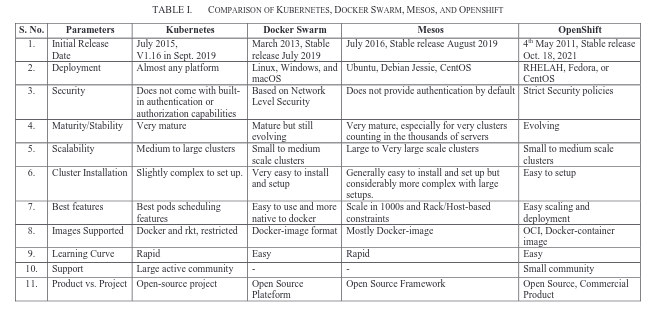
\includegraphics[width=\linewidth]{imagenes/Comparison_Openshift.png}
    \caption{Comparison of Kubernetes, Docker Swarm, Mesos and OpenShift}
    \label{fig:server2}
\end{figure}


\newpage
\subsection*{Análisis Comparativo}
Ahora damos una corporación en forma de tabla donde se detallan las herramientas y la relación con mis objetivos para este proyecto.

\begin{center}
    \begin{tabularx}{\linewidth}{|l|X|X|X|X|} % Ajusta el 'X' para las columnas que necesitan auto-ajuste
        \hline
        \textbf{Características} & \textbf{Docker Swarm} & \textbf{Kubernetes} & \textbf{OpenShift} & \textbf{Apache Mesos} \\
        \hline
        Compatibilidad con HPC & Limitada & Alta, ampliamente adoptado & Alta, diseñado para entornos empresariales & Alta, especialmente en Big Data \\
        \hline
        Despliegue de LLMs & Posible, requiere configuración extra & Ideal para despliegue de aplicaciones complejas, incluyendo LLMs. & Adecuado para LLMs, seguridad reforzada & Escalable, pero no especializado en LLMs \\
        \hline
        Herramientas de SRE & Limitadas & Requiere configuración, pero muy potentes & Integradas (logging, autoscaling, RBAC) & Básicas, depende de configuración manual \\
        \hline
        Escalabilidad & Buena, pero menos flexible & Excelente, diseñado para escalabilidad horizontal y vertical. & Excelente, con alta disponibilidad & Excelente, enfocado en escalabilidad masiva \\
        \hline
        Integración con CI/CD & Requiere herramientas externas & Amplia integración con Jenkins, GitLab... & CI/CD nativo y pipelines predefinidos & Limitada \\
        \hline
        Facilidad de uso & Alta, interfaz simple & Complejo pero flexible y potente & Equilibrado, interfaz gráfica útil & Complejo, curva de aprendizaje elevada \\
        \hline
    \end{tabularx}
\end{center}

\newpage
\begin{multicols*}{2}

\subsection*{Conclusión}
Cada una de las herramientas analizadas tiene sus puntos fuertes y débiles frente a los criterios definidos: desarrollo activo, rendimiento HPC, flexibilidad, herramientas SRE y facilidad de integración CI/CD.

Kubernetes destaca por su flexibilidad y una comunidad activa muy grande. Docker Swarm es fácil de usar y está bien integrado en el ecosistema Docker, pero está más enfocado en aplicaciones de menor escala. Apache Mesos es excelente para manejar grandes clústeres, pero su comunidad reducida y la falta de integración con herramientas sobre SRE lo hacen menos atractivo para este proyecto. Finalmente, OpenShift, basado en Kubernetes, combina seguridad, facilidad de despliegue y automatización, y es una solución de nivel empresarial ideal para entornos HPC.

OpenShift incorpora herramientas de SRE que permiten el monitoreo, el registro de eventos y el escalado automático, facilitando una gestión proactiva de los recursos y la detección temprana de fallos. Estos aspectos son clave para garantizar la disponibilidad y el rendimiento tanto del servidor HPC como de los modelos LLM. Diseñado para entornos empresariales exigentes, permite gestionar aplicaciones complejas con alta eficiencia y continuidad operativa mediante mecanismos de recuperación y escalado dinámico.

Además, su compatibilidad nativa con pipelines de CI/CD agiliza la entrega continua de software, lo que resulta fundamental en proyectos con despliegues frecuentes. Sus funciones de seguridad integradas, como el control de acceso basado en roles y políticas de aislamiento de contenedores, lo hacen especialmente adecuado para entornos sensibles. Por último, aunque Kubernetes ofrece mayor flexibilidad, OpenShift destaca por su interfaz gráfica y sus herramientas integradas de administración, que simplifican considerablemente el despliegue y mantenimiento de clústeres, reduciendo la complejidad operativa.

Finalmente, tengo que mencionar una motivación personal, la universidad me ha ofrecido un curso específico de formación en OpenShift, lo que facilita el proceso de implementación dentro del proyecto. Esta oportunidad permite consolidar los conocimientos técnicos necesarios para aprovechar al máximo esta plataforma, asegurando así una integración más eficiente y alineada con los objetivos del trabajo.

    \section{Análisis Comparativo de Motores de Inferencia para LLM}
    Al trabajar con LLM, necesitamos sistemas que lo hagan funcionar de manera rápida y eficiente, especialmente para aprovechar al máximo la infraestructura en la que están desplegados. En este contexto, los motores de inferencia desempeñan un papel clave, actuando como los “cerebros logísticos” que gestionan estos modelos. Su función principal es organizar y optimizar los recursos disponibles de la forma más eficiente, asegurando así un rendimiento óptimo y un uso inteligente de la infraestructura.
    
    En el presente análisis se exploran tres opciones destacadas: vLLM, TensorRT-LLM de NVIDIA y Text Generation Inference (TGI) de Hugging Face.
    
    \subsection*{vLLM}
    vLLM es un framework de alto rendimiento y código abierto. Fue desarrollado originalmente en la Universidad de California en Berkeley, en colaboración con Neural Magic, empresa que lideraba su mantenimiento y dessarrollo. Desde diciembre de 2024, Red Hat adquirió Neural Magic, convirtiéndose en el principal impulsor comercial del proyecto. A pesar de este cambio, vLLM sigue siendo un proyecto open source, con desarrollo activo en colaboración con la comunidad y la universidad donde se originó
    
    Su principal innovación es el algoritmo PagedAttention, inspirado en las técnicas de paginación de memoria virtual que usan los sistemas operativos. En lugar de asignar grandes bloques contiguos de memoria para la caché clave-valor (KV) ,una estructura esencial en los LLMs, vLLM organiza la memoria en bloques físicos no contiguos y lógicos. Esto reduce significativamente la fragmentación interna y externa de la memoria, un problema común que limita la cantidad de solicitudes que se pueden procesar al mismo tiempo.
    
    Gracias a esta estrategia, vLLM logra un uso casi perfecto de la memoria de la caché KV, con prácticamente cero desperdicio. Además, permite compartir de manera flexible esta caché entre diferentes solicitudes o incluso dentro de una misma solicitud, como ocurre en tareas de generación paralela o búsqueda por haz (beam search). Esta capacidad de compartir memoria de forma inteligente disminuye aún más el consumo total, lo que posibilita manejar más solicitudes en paralelo y mejora el rendimiento general del sistema.
    
    Las evaluaciones presentadas en el artículo Efficient Memory Management for Large Language Model Serving with PagedAttention muestran que vLLM puede aumentar el rendimiento de modelos como OPT y LLaMA entre 2 y 4 veces en comparación con sistemas avanzados como FasterTransformer y Orca, manteniendo niveles de latencia similares. Estas mejoras son especialmente notables en escenarios desafiantes, como secuencias de texto largas, modelos de mayor tamaño y algoritmos de decodificación complejos.
    
    \subsection*{TensorRT-LLM - NVIDIA}
    Pasemos ahora a TensorRT-LLM, desarrollado por NVIDIA y optimizado específicamente para sus GPUs, como las A100 o H100. Este motor está diseñado para ofrecer el máximo rendimiento en hardware NVIDIA, utilizando técnicas avanzadas como la fusión de capas, la cuantización y la ejecución optimizada de kernels CUDA. Estas optimizaciones permiten alcanzar velocidades de inferencia significativamente superiores a las de otros motores más generales.
    
    Por ejemplo, en benchmarks oficiales, TensorRT-LLM logró un rendimiento de aproximadamente 3,679 tokens por segundo con el modelo GPT-J de 6 mil millones de parámetros sobre una GPU A100 de 80 GB . En comparación, vLLM alcanza aproximadamente 714 tokens por segundo con modelos equivalentes como LLaMA-7B en una A100 de 40 GB. Esta diferencia se debe principalmente a las optimizaciones de bajo nivel específicas para GPUs NVIDIA que implementa TensorRT-LLM.
    
    Sin embargo, esta especialización tiene un costo: TensorRT-LLM está limitada a GPUs NVIDIA y requiere que los modelos 

    se conviertan a un formato especial llamado TensorRT Engine, lo que puede añadir complejidad al proceso. Aunque es una herramienta poderosa para quienes ya trabajan con hardware NVIDIA, su falta de flexibilidad la hace menos versátil en comparación con vLLM.
    
    \subsection*{Text Generation Inference (TGI) - Hugging Face}
    Por otro lado, TGI, creado por Hugging Face, se destaca por su capacidad para manejar textos extremadamente largos de manera eficiente.Utiliza técnicas que le permiten recordar información previa sin necesidad de recalcular todo desde cero, lo que ahorra memoria y acelera las respuestas. En pruebas con prompts de más de 200,000 tokens, TGI generó respuestas en solo 2 segundos, mientras que vLLM tardó 27.5 segundos. Además, en una GPU NVIDIA L4, TGI puede manejar hasta 30k tokens, tres veces más que vLLM en configuraciones similares.

    TGI también es muy fácil de usar: con solo especificar el nombre de un modelo de Hugging Face, está lista para funcionar, sin configuraciones complicadas. Aunque está optimizada principalmente para GPUs NVIDIA, su buen desempeño en hardware con recursos limitados la hace atractiva para usuarios con equipos más modestos.

\end{multicols*}

\newpage

\subsection*{Análisis Comparativo}
\begin{center}
\begin{tabularx}{\linewidth}{|l|X|X|X|}
    \hline
    \textbf{Característica} & \textbf{vLLM} & \textbf{TensorRT-LLM (NVIDIA)} & \textbf{Text Generation Inference (TGI) (Hugging Face)} \\
    \hline
    ¿Open Source? & Si & No, es de Nvidia & Si \\
    \hline
    Hardware Principal & Amplia gama de GPUs (NVIDIA, AMD, etc.) & GPUs NVIDIA (optimizado para) & Principalmente GPUs NVIDIA (ejemplo con L4) \\
    \hline
    Optimización Clave & PagedAttention, ahora con soporte de Red Hat & Optimización a nivel de kernel, fusión de capas, gestión dinámica de memoria & Optimización de memoria para prompts largos, retención de contexto, estructuras de datos eficientes \\
    \hline
    Facilidad de Uso & API de Python sencilla, servidor compatible con OpenAI API & Requiere conversión de modelos a formato TensorRT Engine & Cero configuración para la mayoría de los casos, basado en ID de modelo de Hugging Face \\
    \hline
    Rendimiento (vs. vLLM) & 2-4x más rápido que Orca; generalmente más lento que TensorRT-LLM en NVIDIA & Generalmente más rápido y energéticamente eficiente en GPUs NVIDIA & Hasta 13x más rápido en prompts largos (>200k tokens), triplica la capacidad de tokens \\
    \hline
    Manejo de Prompts Largos & Gestión eficiente de memoria KV ayuda & Optimizado para reducir latencia y huella de memoria & Optimizado significativamente, triplica la capacidad de tokens \\
    \hline
    Flexibilidad Hardware & Alta & Limitada a NVIDIA & Principalmente NVIDIA, buena optimización para hardware limitado \\
    \hline
\end{tabularx}
\end{center}
 
\newpage
\subsection*{Conclusión}
\begin{multicols*}{2}

Tras evaluar vLLM, TensorRT-LLM y TGI, vLLM se destaca como la opción más equilibrada en términos de eficiencia, flexibilidad y facilidad de integración. Su algoritmo PagedAttention optimiza el uso de la memoria GPU, permitiendo gestionar múltiples solicitudes concurrentes sin desperdicio de recursos. Por ejemplo, en pruebas con el modelo OPT-13B, vLLM procesó hasta 2.2 veces más solicitudes simultáneas que Orca (Oracle) y 4.3 veces más que Orca (Max), manteniendo latencias similares.

Además, su compatibilidad con hardware diverso (GPUs NVIDIA, AMD, CPUs, TPUs), su naturaleza open source, y el impulso actual de Red Hat como principal contribuidor tras la adquisición de Neural Magic, refuerzan su sostenibilidad a largo plazo y su capacidad de innovación.

Un aspecto especialmente relevante para este Trabajo de Fin de Grado es que vamos a trabajar sobre Red Hat OpenShift como plataforma de orquestación. En este entorno, vLLM está mejor documentado e integrado que otras opciones. Red Hat ha anunciado soporte directo de vLLM en su ecosistema de IA empresarial (incluido en OpenShift AI), facilitando así tanto el despliegue como el escalado automático, el control de recursos y la integración con pipelines de MLOps.

Aunque TensorRT-LLM ofrece un rendimiento superior en hardware NVIDIA y TGI tiene ventajas notables en escenarios con prompts extremadamente largos, vLLM proporciona un rendimiento estable y adaptable, siendo ampliamente utilizado en entornos reales y cada vez más estandarizado. En consecuencia, es la opción más práctica y escalable para un proyecto que busca eficiencia sin comprometer portabilidad ni simplicidad operativa.    

\section{Análisis Comparativo de Modelos LLM}
Una vez elegida OpenShift como plataforma para la gestión del proyecto, el siguiente paso fue determinar qué modelos de lenguaje (LLM) resultaban más adecuados para su implementación en entornos de computación de alto rendimiento (HPC) mediante vLLM. Para ello, se analizaron modelos reconocidos como ChatGPT, Google Gemini, LLaMA y DeepSeek.
\begin{figure}[H]
    \centering
    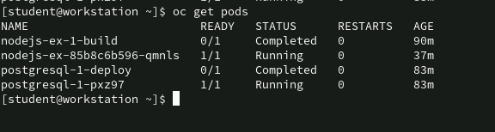
\includegraphics[width=\linewidth]{imagenes/image22.png}
    \caption{}
    \label{fig:server4}
\end{figure}


La evaluación se basó en tres enfoques complementarios. En primer lugar, se revisaron estudios técnicos detallados publicados en artículos científicos, en los cuales se aplicó una metodología zero-shot para tareas de extracción de relaciones en chino, utilizando métricas objetivas como precisión, recall, F1-score y latencia. En segundo lugar, se consideraron resultados normalizados en pruebas estandarizadas ampliamente reconocidas, como MMLU, SAT, LSAT, GRE, TOEFL o GMAT, que permiten medir la capacidad de los modelos en tareas académicas complejas y diversas. Por último, se incorporó la información procedente de Chatbot Arena, una plataforma de evaluación comunitaria basada en comparaciones por pares y votaciones entre modelos, que genera puntuaciones mediante el sistema Elo a partir de más de 2,8 millones de enfrentamientos. Esta combinación de enfoques permite integrar la precisión técnica, el rendimiento en escenarios exigentes y la experiencia práctica de los usuarios en un único análisis comparativo.
\begin{figure}[H]
    \centering
    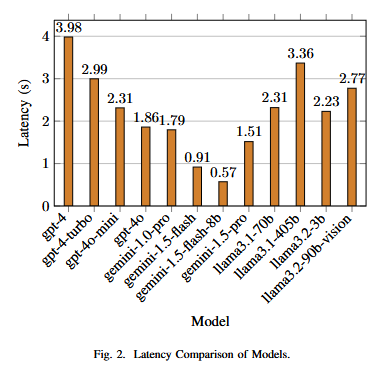
\includegraphics[width=\linewidth]{imagenes/image15.png}
    \caption{}
    \label{fig:server3}
\end{figure}
Chatbot Arena, en particular, resultó ser una herramienta valiosa para evaluar la percepción práctica de los usuarios sobre estos modelos. Con más de 24 millones de votos, la plataforma genera clasificaciones generales mediante un sistema Elo, ofreciendo una visión actualizada y dinámica. Este enfoque destaca diferencias en fluidez, relevancia y coherencia que, en ocasiones, no se evidencian en pruebas más controladas. Por ejemplo, las puntuaciones Elo indican que ChatGPT, especialmente en su versión GPT-4o, alcanza una calificación destacada de aproximadamente 1406, superando a otros modelos y mostrando coherencia con los buenos resultados obtenidos en los análisis técnicos.


\subsection*{ChatGPT}
ChatGPT, desarrollado por OpenAI, alcanzó una gran popularidad tras su lanzamiento en noviembre de 2022. Inicialmente construido sobre GPT-3.5 y posteriormente evolucionado a GPT-4, este modelo emplea una arquitectura de transformador perfeccionada mediante técnicas como el aprendizaje por refuerzo con retroalimentación humana (Reinforcement Learning from Human Feedback, RLHF). Estas mejoras permiten ofrecer respuestas claras, coherentes y adaptadas al contexto, lo que lo ha convertido en una herramienta destacada para la conversación, la redacción de textos y el soporte en programación.

En el estudio de extracción de relaciones en chino, por ejemplo, ChatGPT alcanzó una precisión de aproximadamente 0,363 y un F1-score de 0,358, lo que demuestra su capacidad para generar contenido relevante. No obstante, esta capacidad conlleva un coste: su elevado consumo computacional puede provocar demoras. En el caso de GPT-4, las respuestas pueden tardar hasta 3,98 segundos. En plataformas como Chatbot Arena, los usuarios elogian la calidad de sus respuestas, aunque algunos han señalado que la espera puede representar un inconveniente cuando se requiere inmediatez.

\subsection*{Google Gemini}
Google Gemini, desarrollado por el equipo de DeepMind de Google, fue lanzado en 2023. Este modelo se caracteriza por su arquitectura multimodal, que le permite procesar y generar simultáneamente distintos tipos de datos, incluyendo texto, imágenes y código. En el documento (2502.05694v1.pdf) se muestra que algunas variantes de Gemini, como gemini-1.5-flash-8b, presentan latencias extremadamente bajas, en torno a 0,57 segundos, y precisiones que varían entre 0,295 (gemini-1.0-pro) y 0,354 (gemini-1.5-pro). Esta combinación resulta especialmente atractiva para aplicaciones en tiempo real, donde la velocidad de respuesta es un factor crítico.

Además, las evaluaciones de Chatbot Arena destacan la rapidez de Gemini, situándose en posiciones altas en términos de velocidad. Sin embargo, en comparativas centradas exclusivamente en contenido textual, sus puntuaciones Elo suelen ser algo inferiores a las de ChatGPT, lo que sugiere un compromiso entre velocidad y precisión.

\subsection*{LLaMA}
LLaMA, acrónimo de Large Language Model Meta AI, es un modelo desarrollado por Meta y lanzado en febrero de 2023. Las evaluaciones técnicas en el estudio de extracción de relaciones indican que LLaMA presenta un rendimiento inferior en este contexto. Por ejemplo, la versión llama3.1-405b obtuvo un F1-score de apenas 0,117 y registró una latencia aproximada de 3,36 segundos. Estos resultados evidencian limitaciones significativas tanto en precisión como en eficiencia, lo que se refleja en los rankings generales (overall) de Chatbot Arena, donde la comunidad de usuarios posiciona a LLaMA en un rango inferior en escenarios de alta exigencia.

Esta baja valoración confirma que, tal como se observa en las métricas experimentales, LLaMA requiere ajustes y mejoras sustanciales para competir eficazmente en aplicaciones críticas.

\subsection*{DeepSeek}
DeepSeek, desarrollado por una empresa emergente china, fue introducido a finales de 2023. Se basa en una arquitectura Mixture-of-Experts (MoE) que activa selectivamente los parámetros necesarios para cada consulta, con el objetivo de optimizar la eficiencia computacional. En el documento (2503.04783v1.pdf) se destacan sus capacidades en tareas de razonamiento, codificación y especialización en ámbitos como la salud, el derecho o las finanzas. Por ejemplo, en la tabla de evaluación general de rendimiento, el modelo DeepSeek R1 obtiene una puntuación de 84,0 en MMLU (Overall), frente a 90,0 de ChatGPT GPT-4o y 87,0 de Gemini 1.5 Pro, lo que indica un rendimiento competitivo, aunque ligeramente inferior en tareas generales de razonamiento y conocimiento.

No obstante, DeepSeek alcanza este nivel de rendimiento mediante una arquitectura mucho más eficiente y orientada, lo que lo convierte en una opción especialmente valiosa en entornos con recursos limitados. En la plataforma Chatbot Arena, los usuarios reconocen su excelente rendimiento en dominios específicos, 

\end{multicols*}

\newpage
\noindent
\begin{minipage}[t]{0.48\textwidth} 
    aunque su capacidad de generalización no alcanza los niveles de los modelos más amplios y carece de capacidades multimodales robustas. A pesar de ello, DeepSeek ha logrado posicionarse como el modelo mejor valorado dentro de la categoría de código abierto, lo que representa un logro significativo para una propuesta relativamente reciente en este mercado competitivo.
\end{minipage}%
\hfill 
\begin{minipage}[t]{0.48\textwidth} 
\end{minipage}

\vspace{1em} 
\noindent 


\begin{figure}[H]
    \centering
    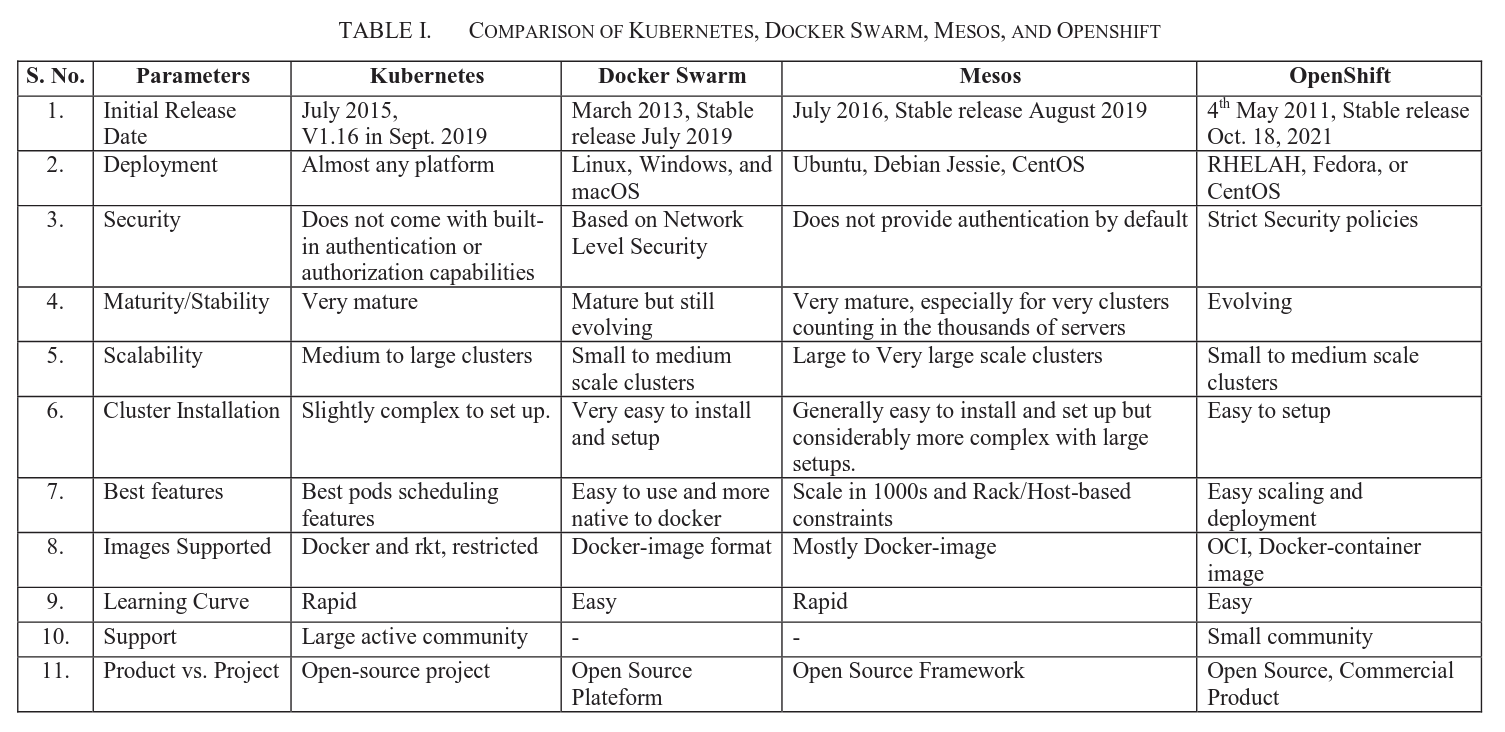
\includegraphics[width=\linewidth]{imagenes/image13.png}
    \caption{}
    \label{fig:server2}
\end{figure}

\newpage

\noindent
\begin{minipage}[t]{0.48\textwidth}
    \subsection*{Analisis Comparativo}
    Una vez presentadas las principales características de los modelos analizados, resulta importante incorporar la evaluación que realiza Chatbot Arena, una plataforma de comparación directa basada en enfrentamientos aleatorios entre modelos. Además del ranking general (Arena Elo), se incluyen benchmarks específicos como MMLU, visto anteriormente (prueba de precisión multitarea en 57 tareas) y Arena-Hard-Auto, una evaluación automática dirigida a modelos adaptados a instrucciones.

    La tabla más reciente de Chatbot Arena, a día que se escribe esta memoria, muestra que ChatGPT-4o y Gemini-2.5-Pro lideran el ranking con valores Elo muy elevados (1406 y 1437, respectivamente), mientras que modelos como DeepSeek-V3 o DeepSeek-R1 presentan rendimientos sólidos pero más discretos (Elo de 1318 y 1359, respectivamente).
\end{minipage}%
\hfill
\begin{minipage}[t]{0.48\textwidth}
    A pesar de ello, DeepSeek-R1 alcanza una puntuación sobresaliente de 90,8 en MMLU, superando a versiones de Gemini 2.0 y situándose cerca del nivel de GPT-4.5 (92,7) o GPT-4o. LLaMA no aparece en los primeros puestos del ranking, aparece con una puntuacion de 1296, siendo el modelo de Llama-3.3-Nemotron-Super-49B-v1, familia de modelo de nvidia pero basado en Llama, se posiciona como el 5 entre modelos open source.

    Esta evaluación empírica confirma que ChatGPT mantiene una posición destacada, no solo por su precisión en entornos controlados, sino también por la preferencia general de los usuarios. Gemini, por su parte, es reconocido por su velocidad y eficiencia multimodal, mientras que DeepSeek se consolida como una opción muy competitiva en precisión multitarea, a pesar de contar con menor visibilidad en el ranking general. En conjunto, la plataforma Chatbot Arena ofrece una perspectiva valiosa al reflejar el rendimiento real y percibido por la comunidad, complementando eficazmente las métricas estáticas tradicionales.
\end{minipage}

\vspace*{0.5em} % Reducido a 0.5em para minimizar el espacio, puedes probar con 0em o un valor negativo si es necesario
\noindent

\begin{figure}[H]
    \centering
    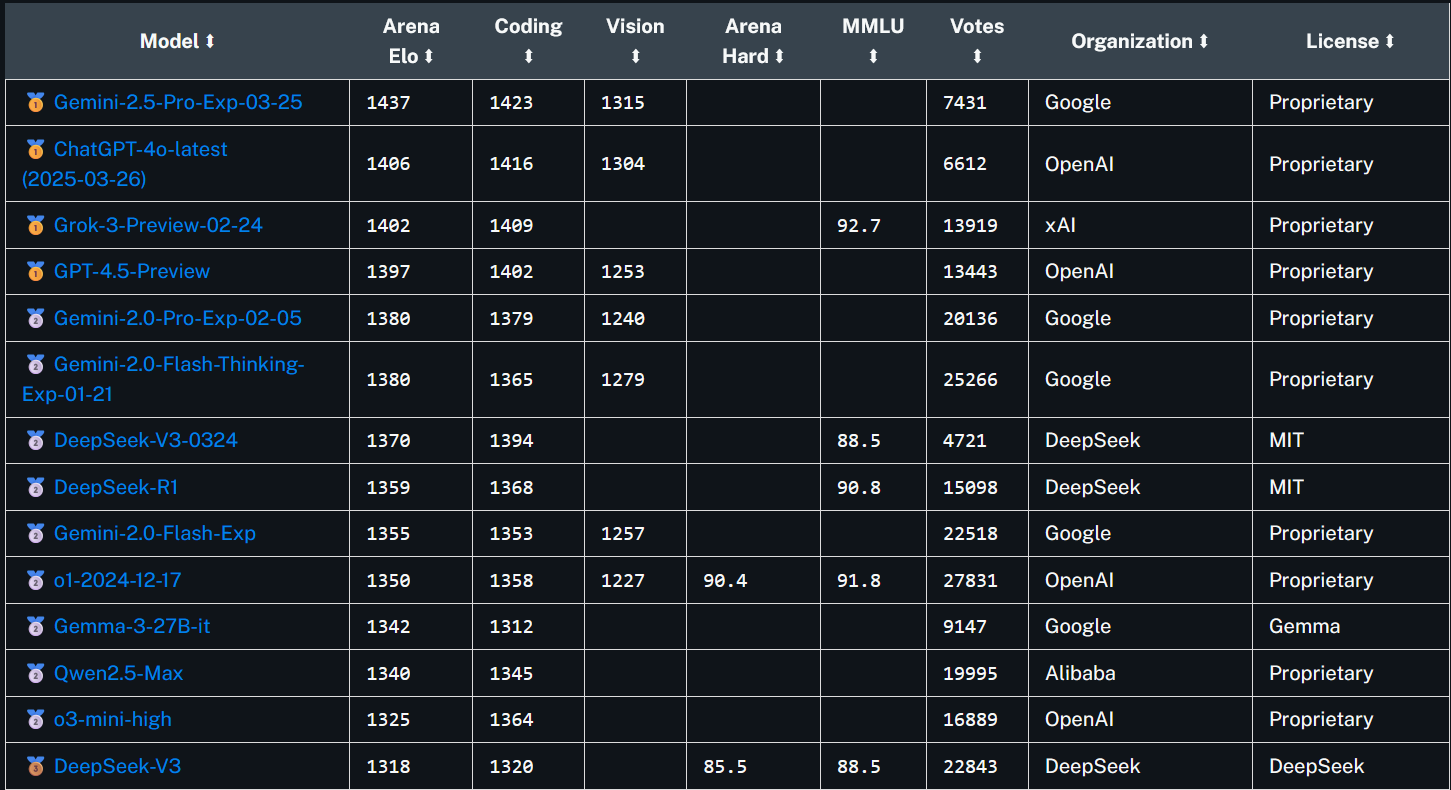
\includegraphics[width=\linewidth]{imagenes/image14.png}
    \caption{}
    \label{fig:server2}
\end{figure}

\newpage
\begin{multicols*}{2}
    \subsection*{Conclusión}
    El análisis realizado permite comprender las fortalezas y limitaciones de los principales modelos LLM en distintos contextos, combinando métricas técnicas con evaluaciones empíricas como las ofrecidas por Chatbot Arena. No obstante, es importante señalar que el ecosistema de modelos evoluciona con gran rapidez: nuevas versiones se publican de forma constante, y un modelo que hoy lidera los rankings puede ser superado en cuestión de semanas.
    
    Aun así, el estudio en profundidad de las características de estos modelos sigue siendo fundamental en el marco de este Trabajo de Fin de Grado, ya que comprender su funcionamiento, eficiencia y adaptación a distintas tareas permite tomar decisiones informadas y anticiparse a futuros desarrollos.
\end{multicols*}




\begin{multicols*}{2}

\chapter{Propuesta}

\section{Propuesta de Trabajo Final de Grado}

Este Trabajo Final de Grado tiene como objetivo la implementación y evaluación de un entorno de computación de alto rendimiento (HPC) para la ejecución de modelos de lenguaje de gran escala (LLM), combinando el uso de contenedores con Podman para el despliegue real sobre GPU y OpenShift Local como entorno de demostración de principios de Site Reliability Engineering (SRE).

Debido a las limitaciones inherentes a OpenShift Local, principalmente la imposibilidad de acceder directamente a la GPU desde su entorno virtualizado, se ha planteado una estrategia dual:
\begin{itemize}
    \item \textbf{Podman (GPU nativa):} Utilizar Podman para el despliegue de modelos LLM en un entorno nativo con GPU y realizar pruebas de rendimiento.
    \item \textbf{OpenShift Local (SRE):} Usar OpenShift Local para simular un entorno de producción y evaluar capacidades avanzadas de SRE como escalado automático, auto-healing y despliegue continuo a partir de repositorios.
\end{itemize}

\section{Fases del Proyecto}

\textbf{Fase de Hardware:}
\begin{itemize}
    \item Montaje físico del servidor, instalación del sistema operativo.
    \item Instalación de controladores y librerías necesarias: NVIDIA Driver, CUDA Toolkit y soporte para contenedores con GPU.
\end{itemize}

\textbf{Fase de Despliegue con Podman (GPU):}
\begin{itemize}
    \item Creación de contenedores con Podman para desplegar un modelo LLM de gran tamaño (ej. DeepSeek) y varios modelos más pequeños.
    \item Configuración del entorno para aprovechar la aceleración por GPU.
    \item Ejecución de pruebas de rendimiento (benchmarks): inferencia, consumo de VRAM, latencias y rendimiento con carga concurrente.
\end{itemize}

\textbf{Fase de Evaluación con OpenShift Local (SRE):}
\begin{itemize}
    \item Instalación y configuración de OpenShift Local.
    \item Despliegue de servicios ligeros desde URLs de GitHub, simulando pipelines DevOps.
    \item Pruebas de capacidades SRE: auto-scaling basado en carga simulada, auto-healing tras fallos intencionados, observabilidad y monitorización de recursos, gestión de actualizaciones y reinicios controlados.
\end{itemize}

\section{Planificación Temporal}

\begin{itemize}
    \item \textbf{Fase Inicial (Semana 1-2):} Montaje del hardware y configuración básica del sistema. Instalación de drivers, CUDA y herramientas necesarias para ejecución con GPU.
    \item \textbf{Fase de Despliegue LLM con Podman (Semanas 3–4):} Despliegue de modelos en contenedores. Ejecución de benchmarks de rendimiento.
    \item \textbf{Fase SRE con OpenShift Local (Semanas 5–6):} Configuración de OpenShift Local. Despliegue de servicios ligeros desde GitHub. Pruebas de escalabilidad y resiliencia.
    \item \textbf{Fase Final (Semana 7-8):} Análisis de resultados. Preparación de la demo y documentación final.
\end{itemize}

\section{Resultados Esperados}

\textbf{Despliegue con GPU (Podman):}
\begin{itemize}
    \item Inferencia funcional de modelos LLM.
    \item Métricas cuantitativas: velocidad de inferencia, uso de recursos, tiempos de respuesta.
\end{itemize}

\textbf{Simulación SRE (OpenShift Local):}
\begin{itemize}
    \item Demostración práctica de escalado automático y auto-healing.
    \item Despliegue automatizado desde repositorios remotos.
    \item Registro de eventos y capacidad de observación del sistema.
\end{itemize}

\section{Objetivo Final}

El objetivo de este proyecto es evaluar la viabilidad y eficiencia del despliegue de modelos de lenguaje de gran escala (LLM) sobre servidores HPC mediante contenedores compatibles con GPU, así como demostrar capacidades clave de Site Reliability Engineering (SRE) mediante OpenShift Local.

Este enfoque dual permite trabajar con modelos reales en el hardware disponible y familiarizarse con tecnologías de orquestación y fiabilidad operativa en entornos simulados. El trabajo se desarrollará con una perspectiva crítica, enfatizando la automatización, resiliencia y optimización del rendimiento, ofreciendo una visión práctica de los retos y soluciones en el despliegue de IA.

Asimismo, este TFG refleja como un roadmap de la experiencia adquirida en el manejo de servidores. Se busca mostrar y consolidar los conocimientos obtenidos durante las prácticas extracurriculares realizadas en Alemania, especialmente en los primeros pasos en la gestión y uso de servidores. Se documentarán tanto los aciertos como los desafíos y los fallos encontrados, detallando el proceso de aprendizaje y las soluciones implementadas a lo largo del desarrollo del proyecto. La intención es ofrecer una referencia formativa útil para futuros estudiantes interesados en el ámbito de la computación de alto rendimiento y la fiabilidad operativa.

\end{multicols*}
\begin{multicols*}{2}

    \chapter{Infraestructura física y puesta a punto}
    
    \section{Primer contacto con la infraestructura física}
    
    El comienzo de este proyecto arrancó con mi primer contacto real con el hardware: la puesta a punto del servidor Dell PowerEdge R7615 en las instalaciones del Centro de Transferencia Tecnológica de la UGR. Todo el proceso se realizó bajo la supervisión de los tutores del TFG, asegurando el cumplimiento de los protocolos de seguridad y las prácticas técnicas establecidas por el centro.
    
    \subsection*{Proceso de instalación}
    
    Antes de nada, como protocolo, se formalizó una solicitud de acceso detallando objetivos y requisitos técnicos, ya que el centro mantiene un control exhaustivo de quién entra y de quién sale, dado que la sala de servidores es un punto crítico de información y servicio para la universidad.
    
    \begin{center}
        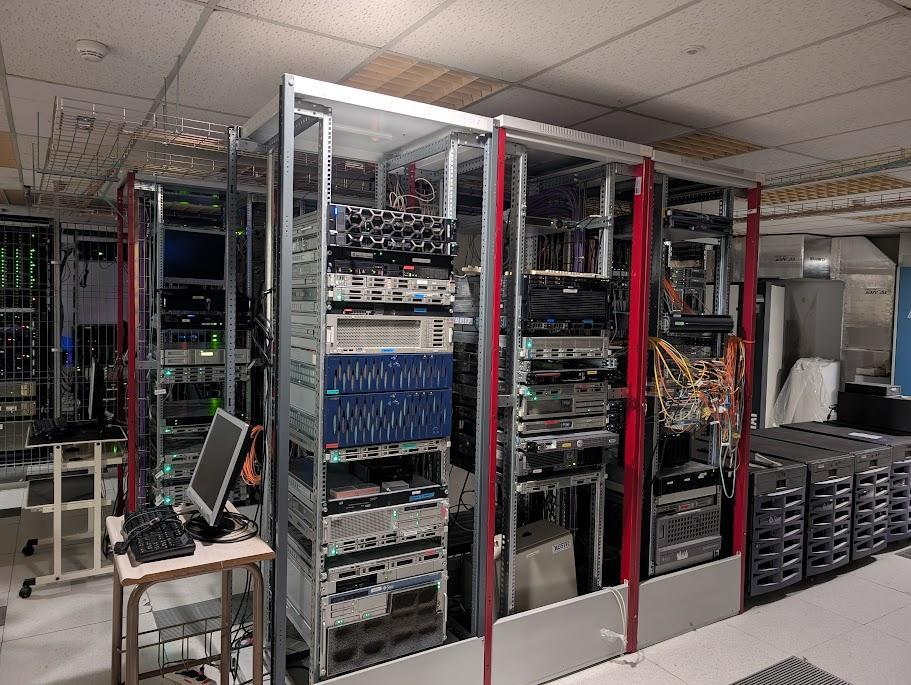
\includegraphics[width=0.95\linewidth]{imagenes/image12.jpg}
        \captionof{figure}{Server Room del CTT de la UGR}
        \label{fig:server-room}
    \end{center}
    
    El montaje se llevó a cabo en un rack estándar de 42U, respetando las distancias mínimas de ventilación (aprox. $\geq$30 cm por delante y por detrás) para evitar el sobrecalentamiento. Las instalaciones cuentan con control de temperatura para proteger los servidores.
    
    \begin{center}
        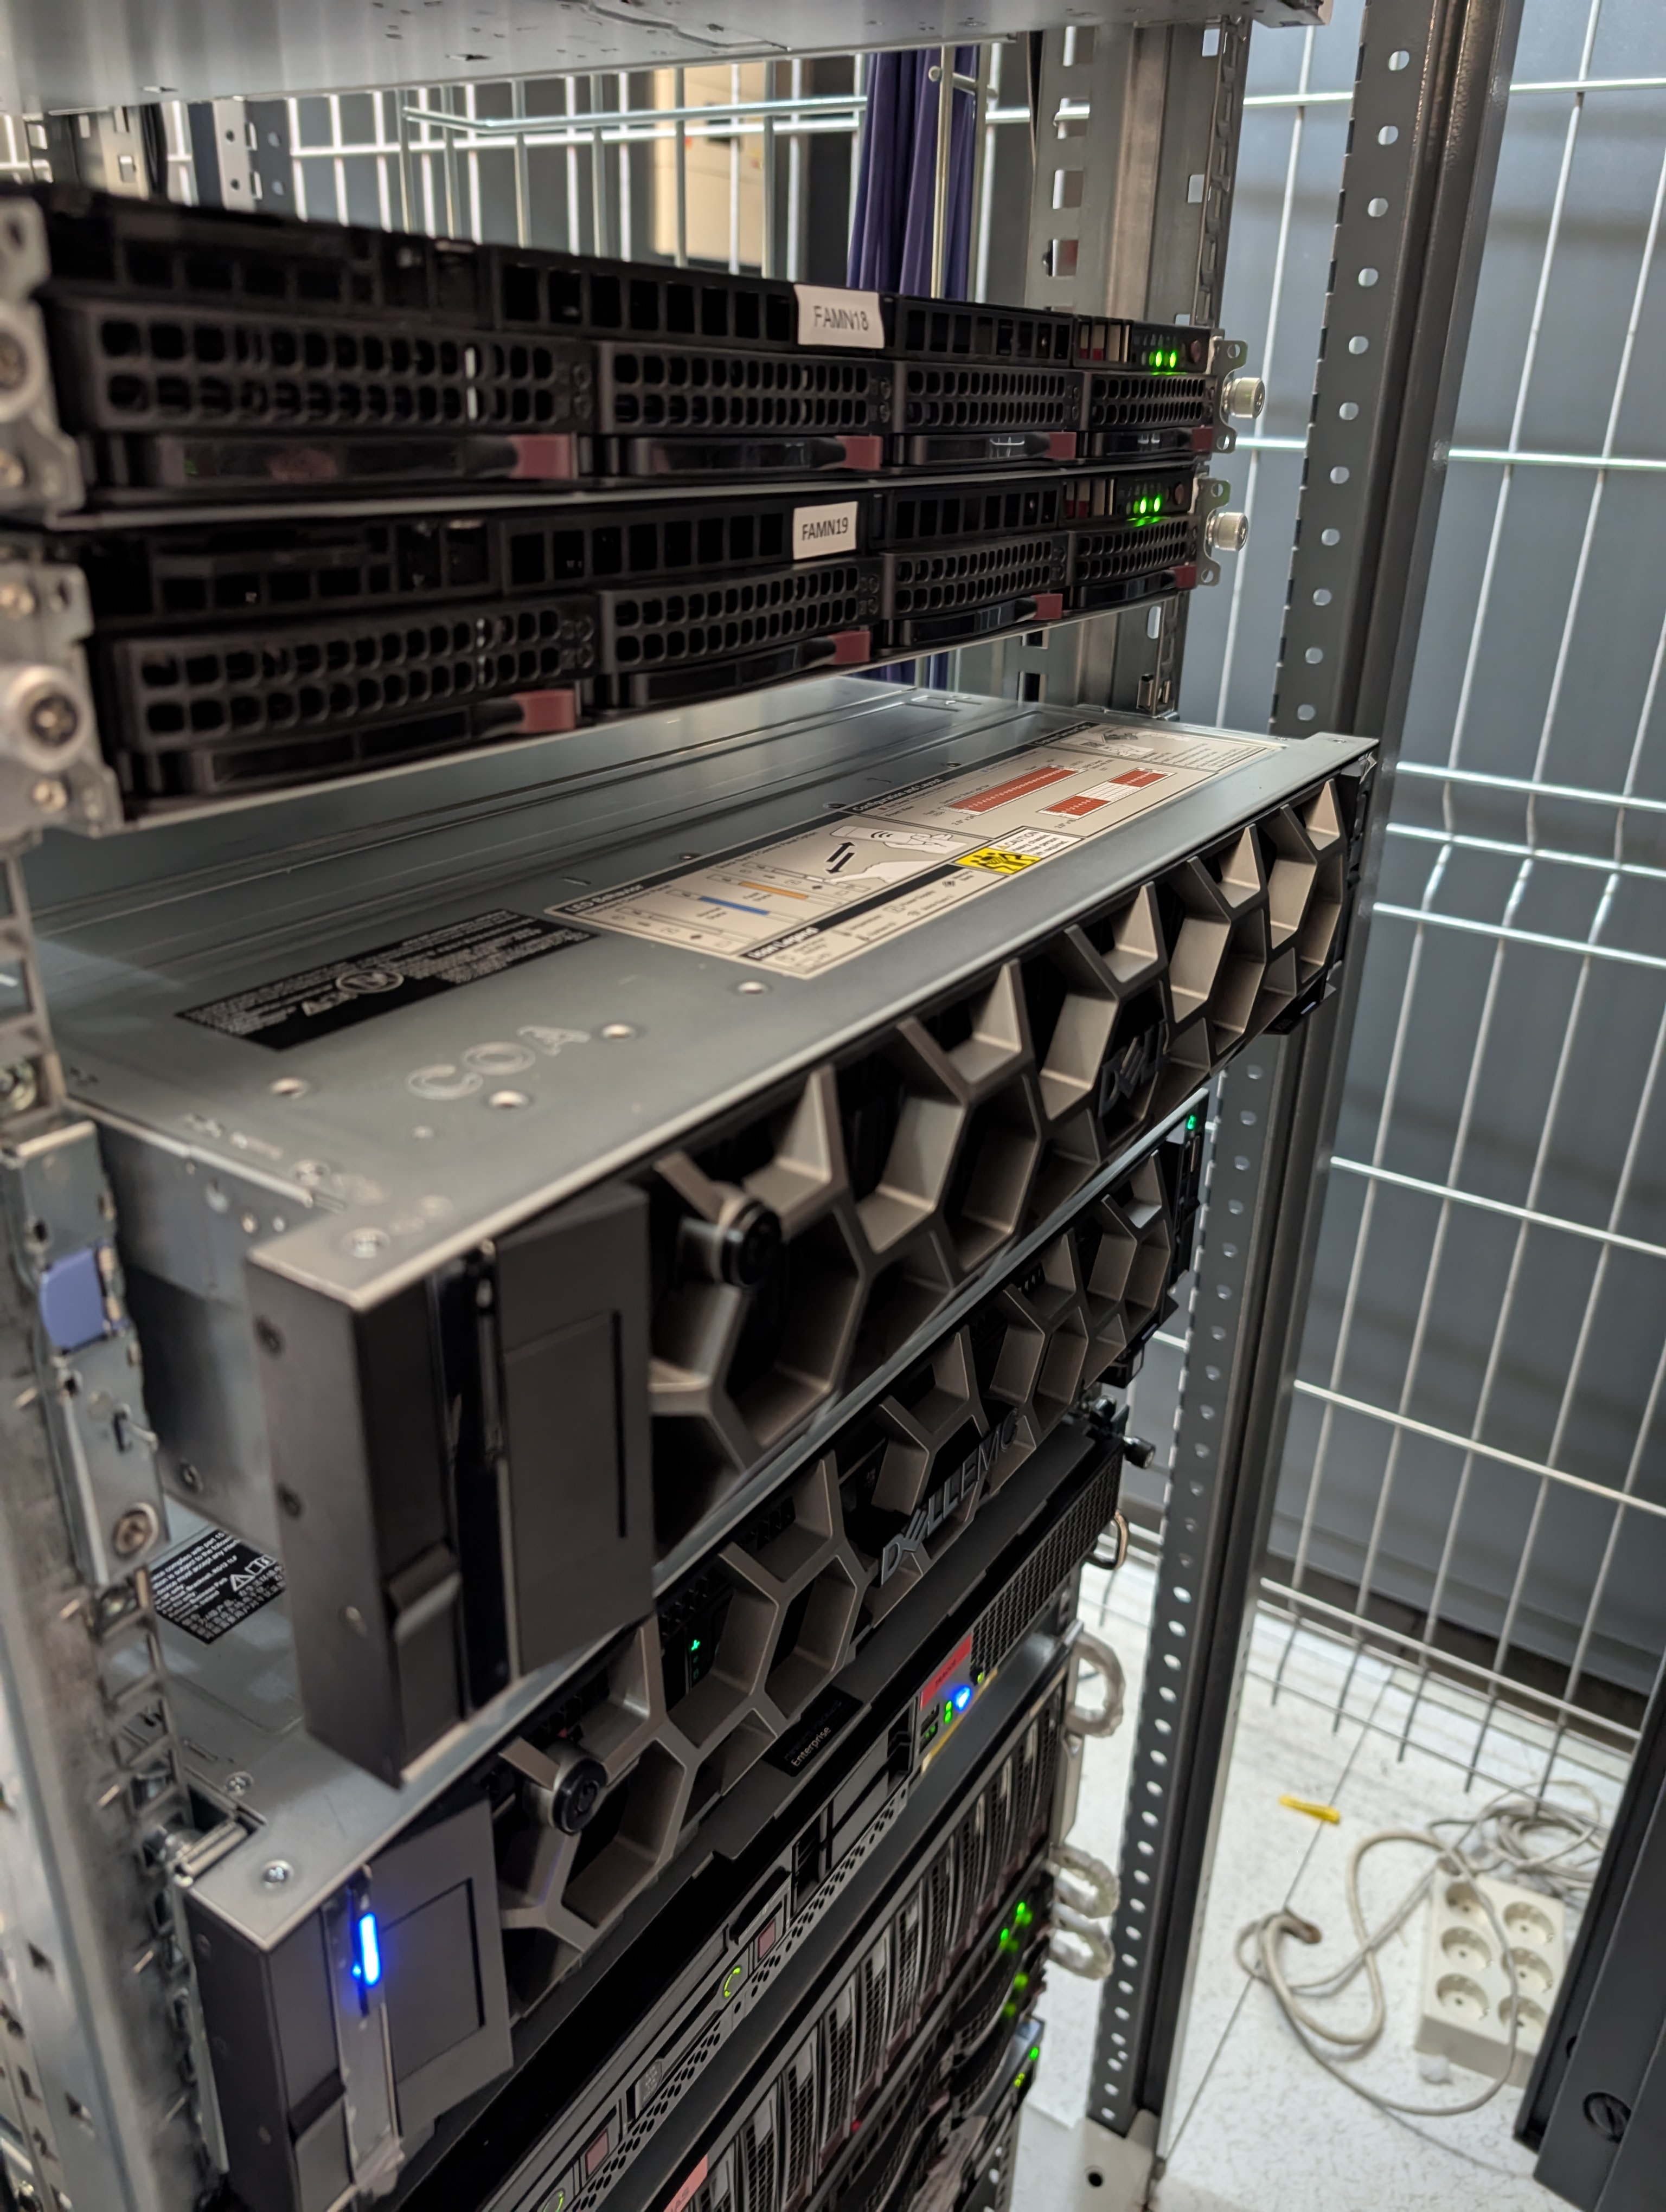
\includegraphics[width=0.85\linewidth]{imagenes/PXL_20250113_100402730.jpg}
        \captionof{figure}{Montaje del servidor Dell PowerEdge R7615}
        \label{fig:montaje-servidor}
    \end{center}
    
    Se instalaron dos fuentes de alimentación separadas y conexiones de red de alta velocidad a 10Gbps, asegurando redundancia y continuidad ante posibles fallos.
    
    Durante la instalación, un pequeño accidente me hizo reflexionar sobre la importancia de los detalles: al desempaquetar el servidor, me corté con el borde de la caja. Mi tutor reaccionó rápidamente con el botiquín, recordándome que, más allá de la tecnología, los pequeños imprevistos pueden afectar el desarrollo de un proyecto.
    
    \begin{center}
        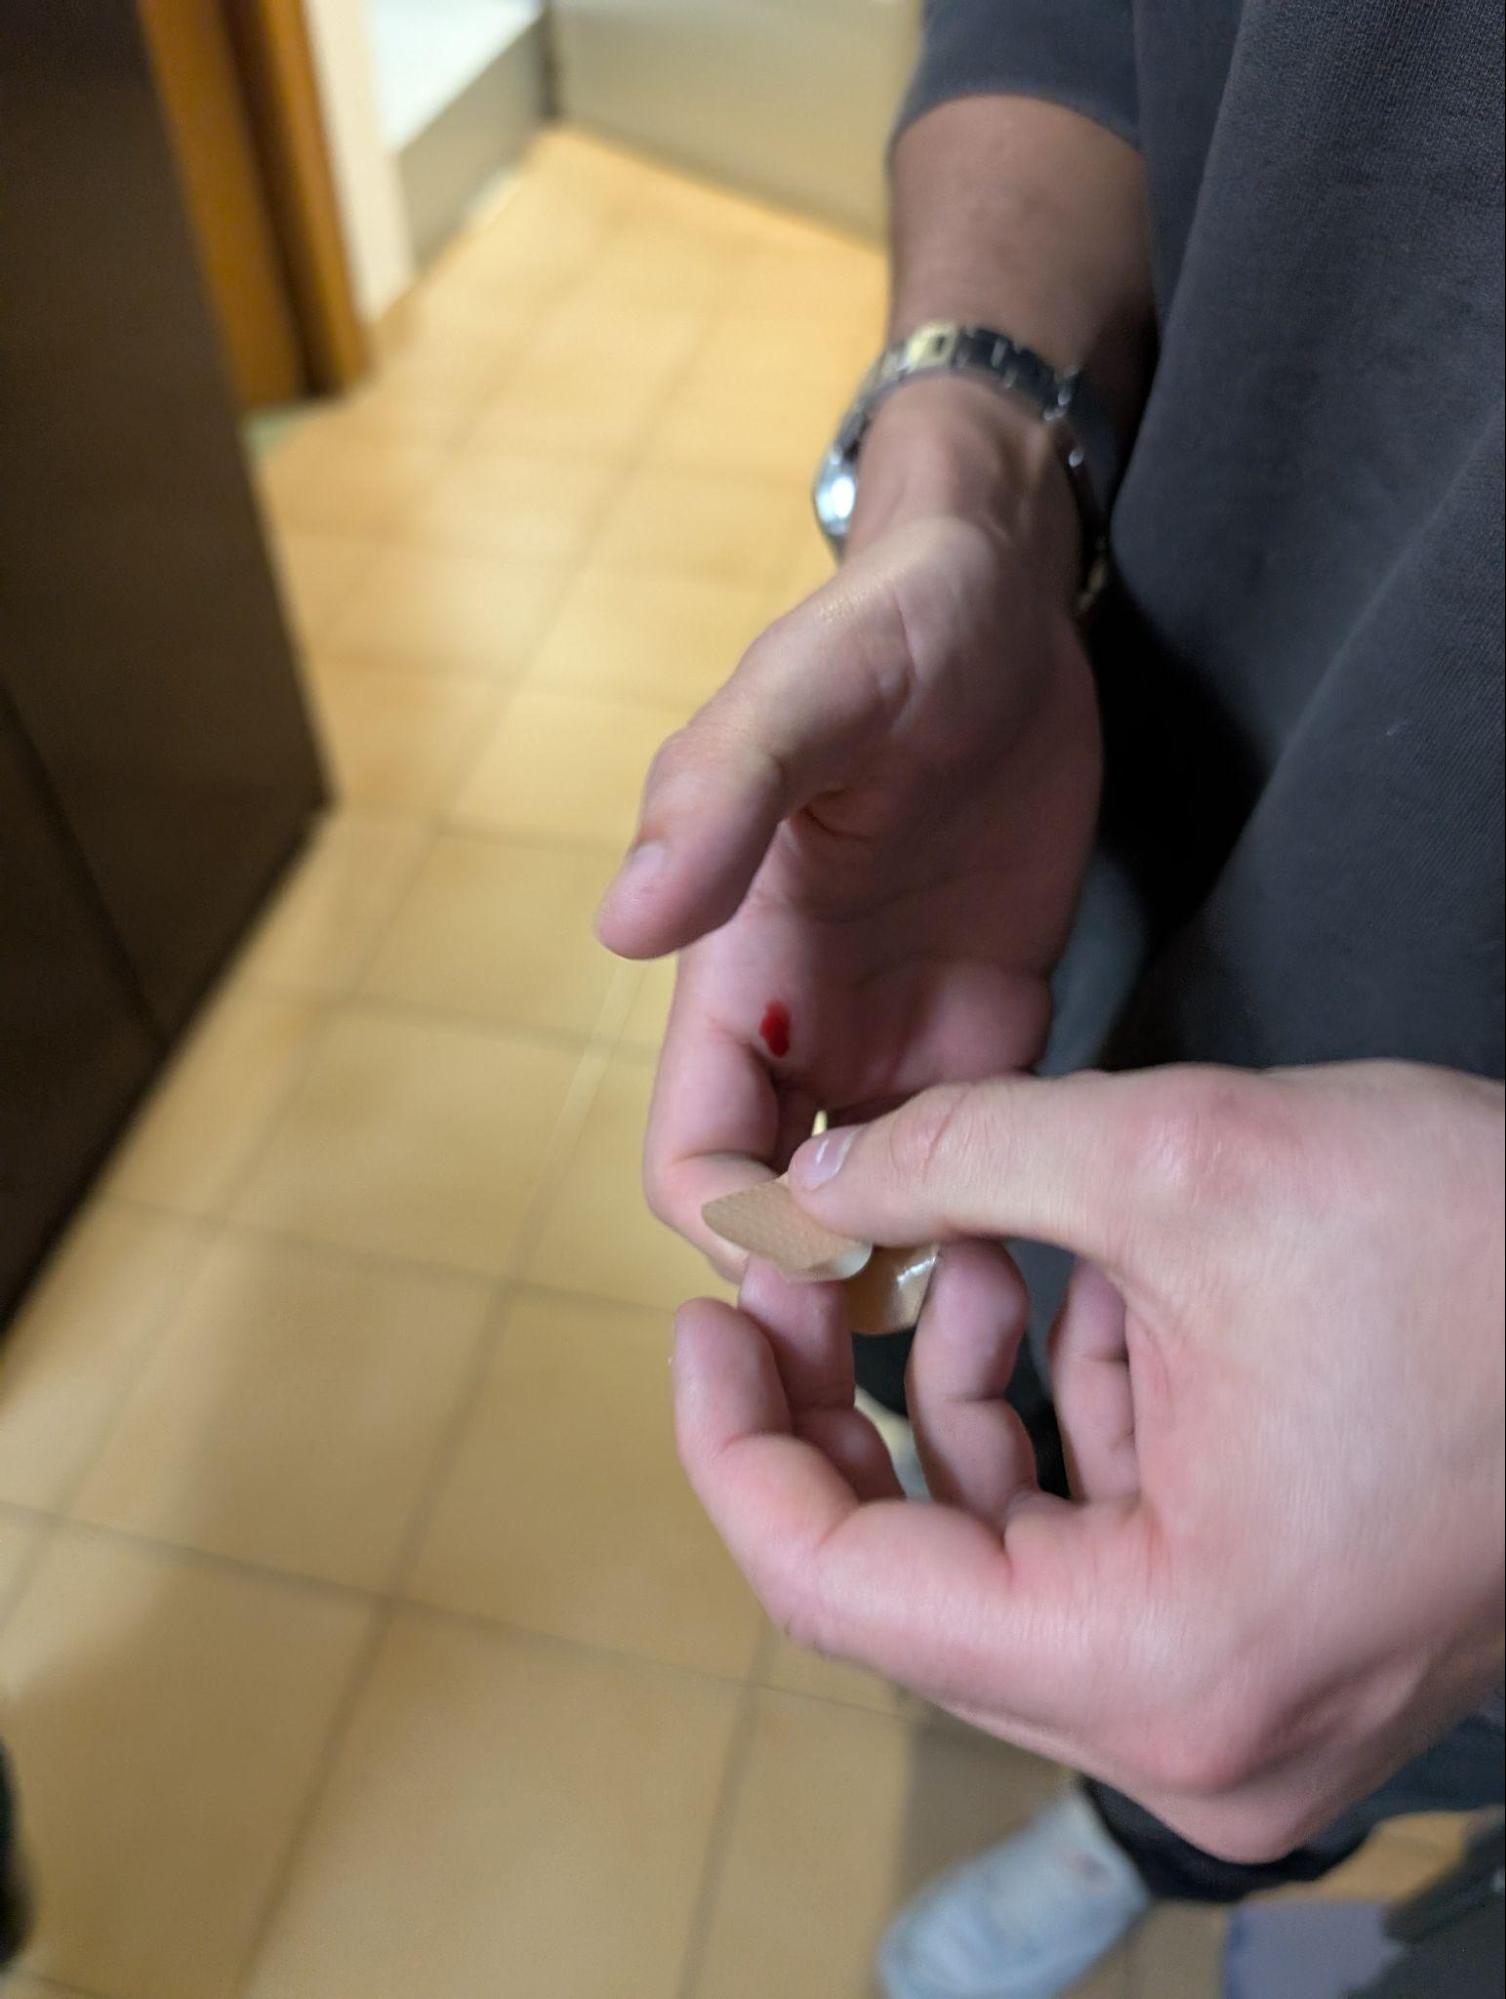
\includegraphics[width=0.95\linewidth]{imagenes/image16.jpg}
        \captionof{figure}{Detalle durante la instalación}
        \label{fig:detalle-instalacion}
    \end{center}
    
    Esta experiencia refuerza la filosofía de Site Reliability Engineering: tan importante es la arquitectura como la capacidad de anticipar y resolver pequeños problemas cotidianos.
    
    \subsection*{Experiencia Práctica y Consideraciones sobre la Instalación}
    
    Cabe señalar que, para el servidor específico de este proyecto, la instalación del sistema operativo y el cableado fueron gestionados por el personal técnico del centro universitario. Sin embargo, este aspecto fue complementado por la experiencia adquirida en mis prácticas Erasmus en la empresa Desion, en Darmstadt, Alemania.
    
    Durante estas prácticas como IT Infrastructure, me responsabilicé del setup de servidores para aplicaciones de IA, incluyendo el montaje físico de componentes como CPU y GPU, y el cableado entre otros. Adicionalmente, di soporte a la automatización de infraestructura, monitoricé el rendimiento y la disponibilidad de sistemas, optimicé pipelines CI/CD y aprendí la importancia de la documentación técnica durante las instalaciones. Para estas tareas, utilicé herramientas como Nagios y Grafana, y perfeccioné mi uso de Docker para el despliegue de servicios empresariales, como la herramienta de anotación de datos CVAT con Traefik.
    
    Un ejemplo clave fue la instalación completa de Ubuntu 22.04 LTS en dos servidores Supermicro. Esta tarea me permitió comprender la importancia de las versiones LTS (Long Term Support), que garantizan actualizaciones de seguridad y estabilidad a largo plazo, frente a versiones más recientes que pueden presentar incompatibilidades. Esta experiencia fue importante para mi desarrollo profesional, ofreciéndome una perspectiva práctica sobre el ciclo de vida del software y las decisiones estratégicas en la selección del sistema operativo, así como una base sólida en el despliegue y mantenimiento de infraestructuras.
    
    \begin{center}
        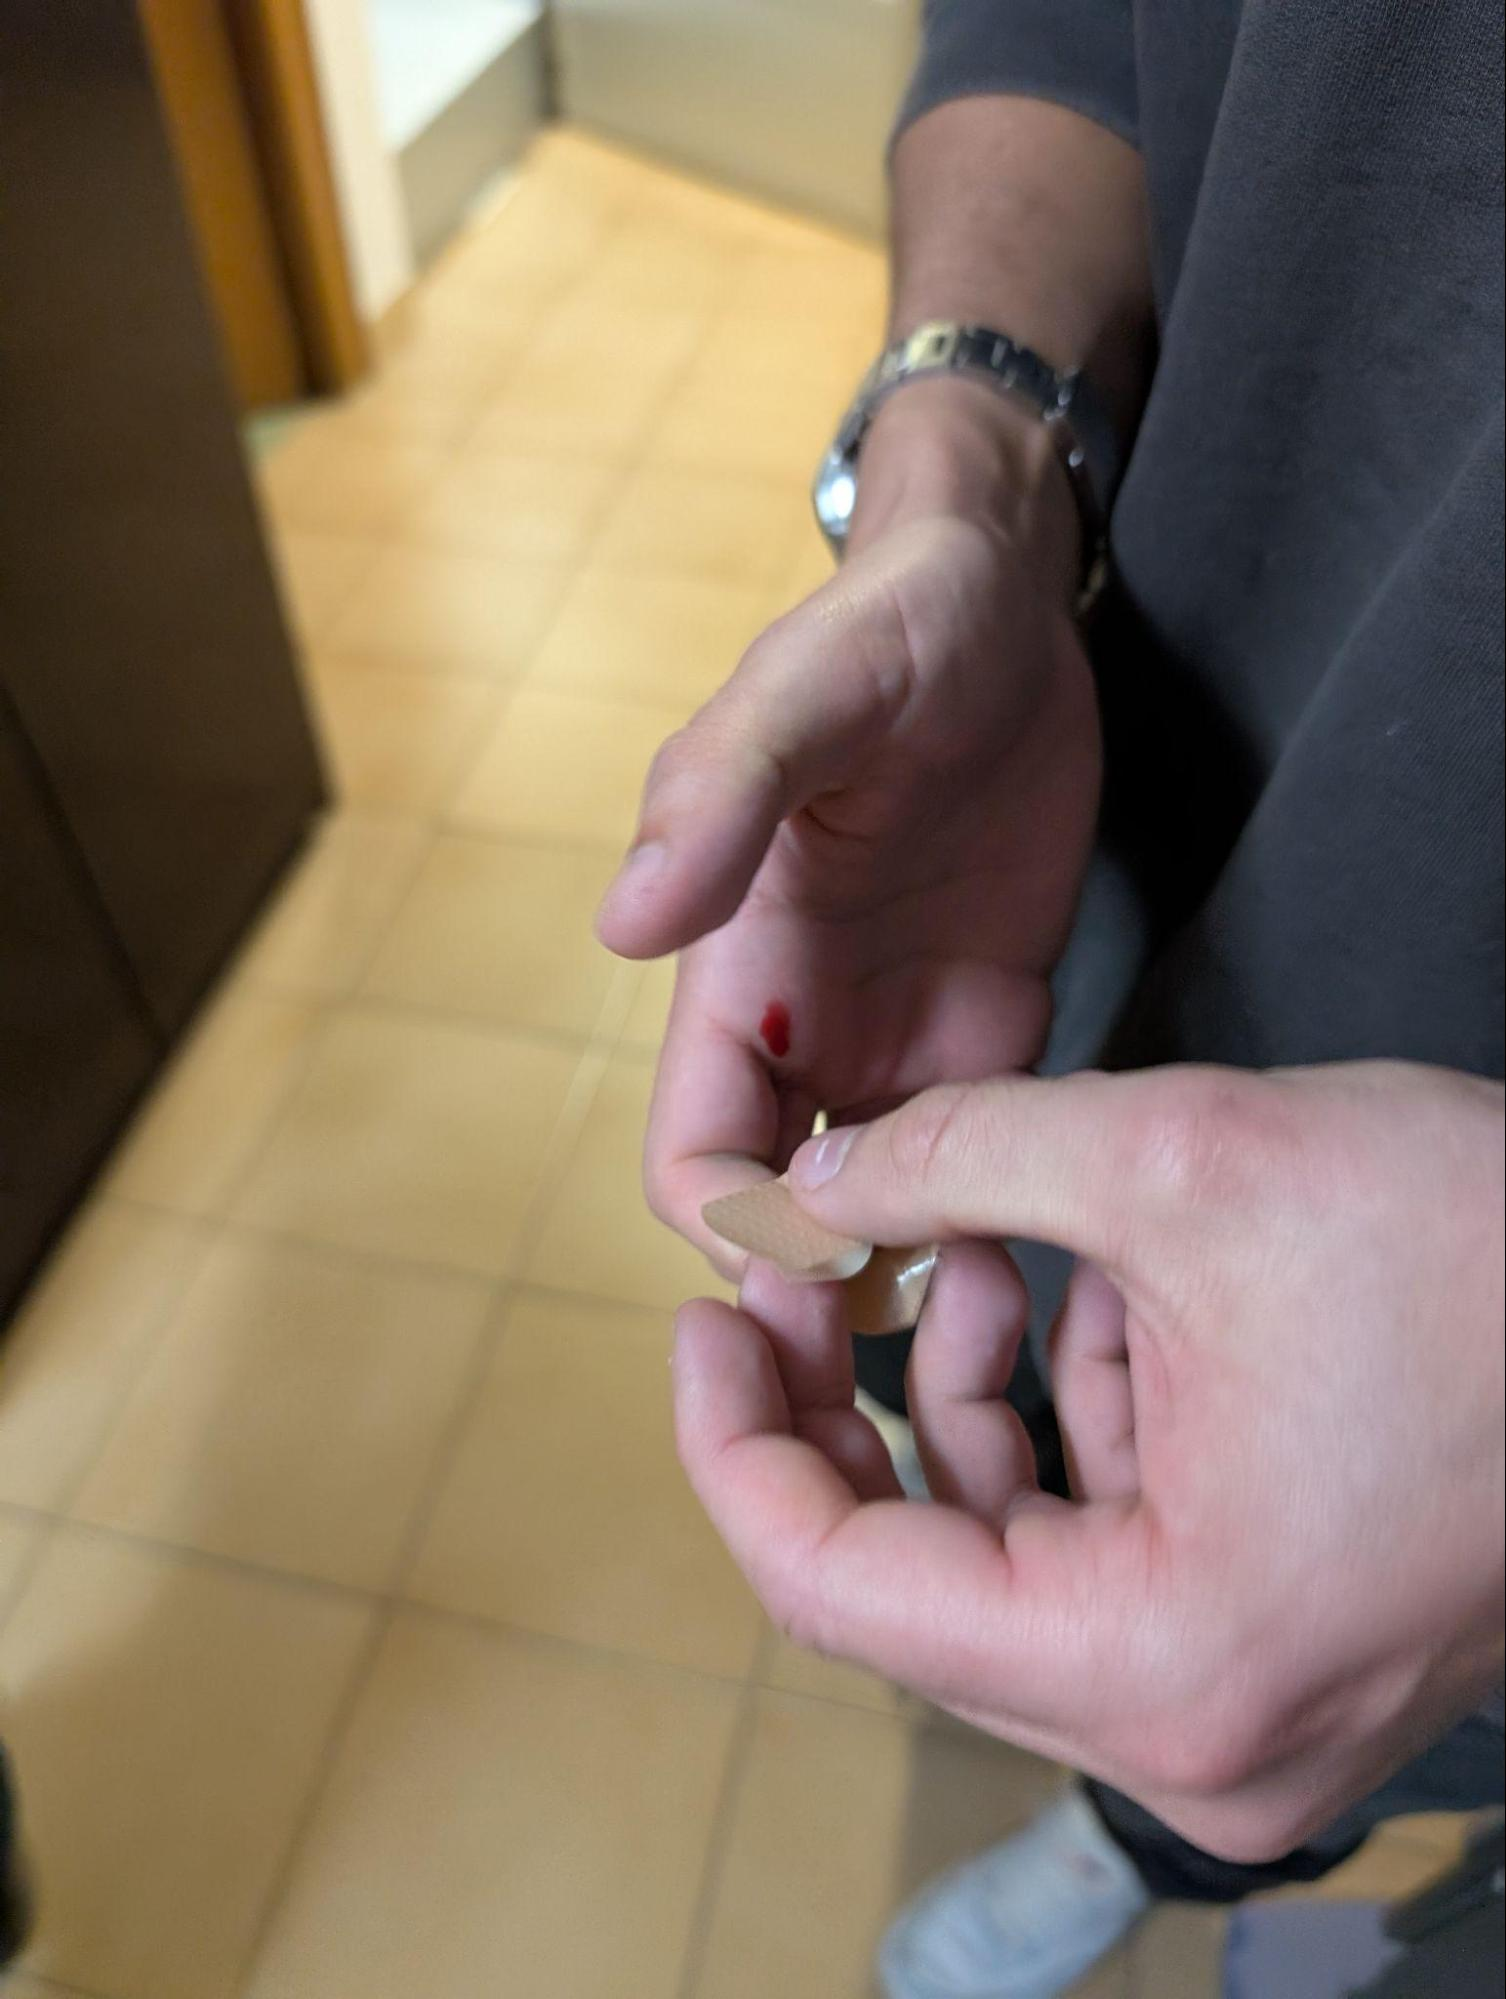
\includegraphics[width=0.95\linewidth]{imagenes/image4.jpg}
        \captionof{figure}{}
        \label{fig:detalle-instalacion2}
    \end{center}

    % cableado + sre

    Otro ejemplo relevante de puesta a punto de infraestructura ocurrió durante mi viaje a Schwechat (Austria), donde realicé la instalación física de los servidores mostrados en la imagen anterior. En esta ocasión, no solo participé en el montaje físico de los equipos en un rack estándar de 42U, sino también en la planificación y ejecución del cableado estructurado, tanto de red como de alimentación. El armario se instaló, y se instalaron los siguientes componentes: un panel de distribución de fibra óptica, dos servidores Dell PowerEdge equipados cada uno con una CPU AMD EPYC y cuatro GPUs NVIDIA L4, un servidor Fujitsu, un SAI APC (Sistema de Alimentación Ininterrumpida) y un switch de red de alto rendimiento con conectividad de 10 Gbps. Todos los equipos se organizaron con gestores de cableado para facilitar el mantenimiento y asegurar una buena ventilación. En cuanto al sistema operativo, instalé Ubuntu 22.04 LTS en ambos servidores Dell y el Futjitsu. 

    Para asegurar la monitorización del sistema, se configuró Nagios en el servidor Fujitsu. Este servidor actuó como nodo de control, vigilando el estado de los otros dos mediante chequeos periódicos de disponibilidad, uso de recursos y estado de red. Esta capacidad de monitorización es clave para anticipar fallos y garantizar la disponibilidad, un principio fundamental del enfoque SRE.

    \begin{center}
        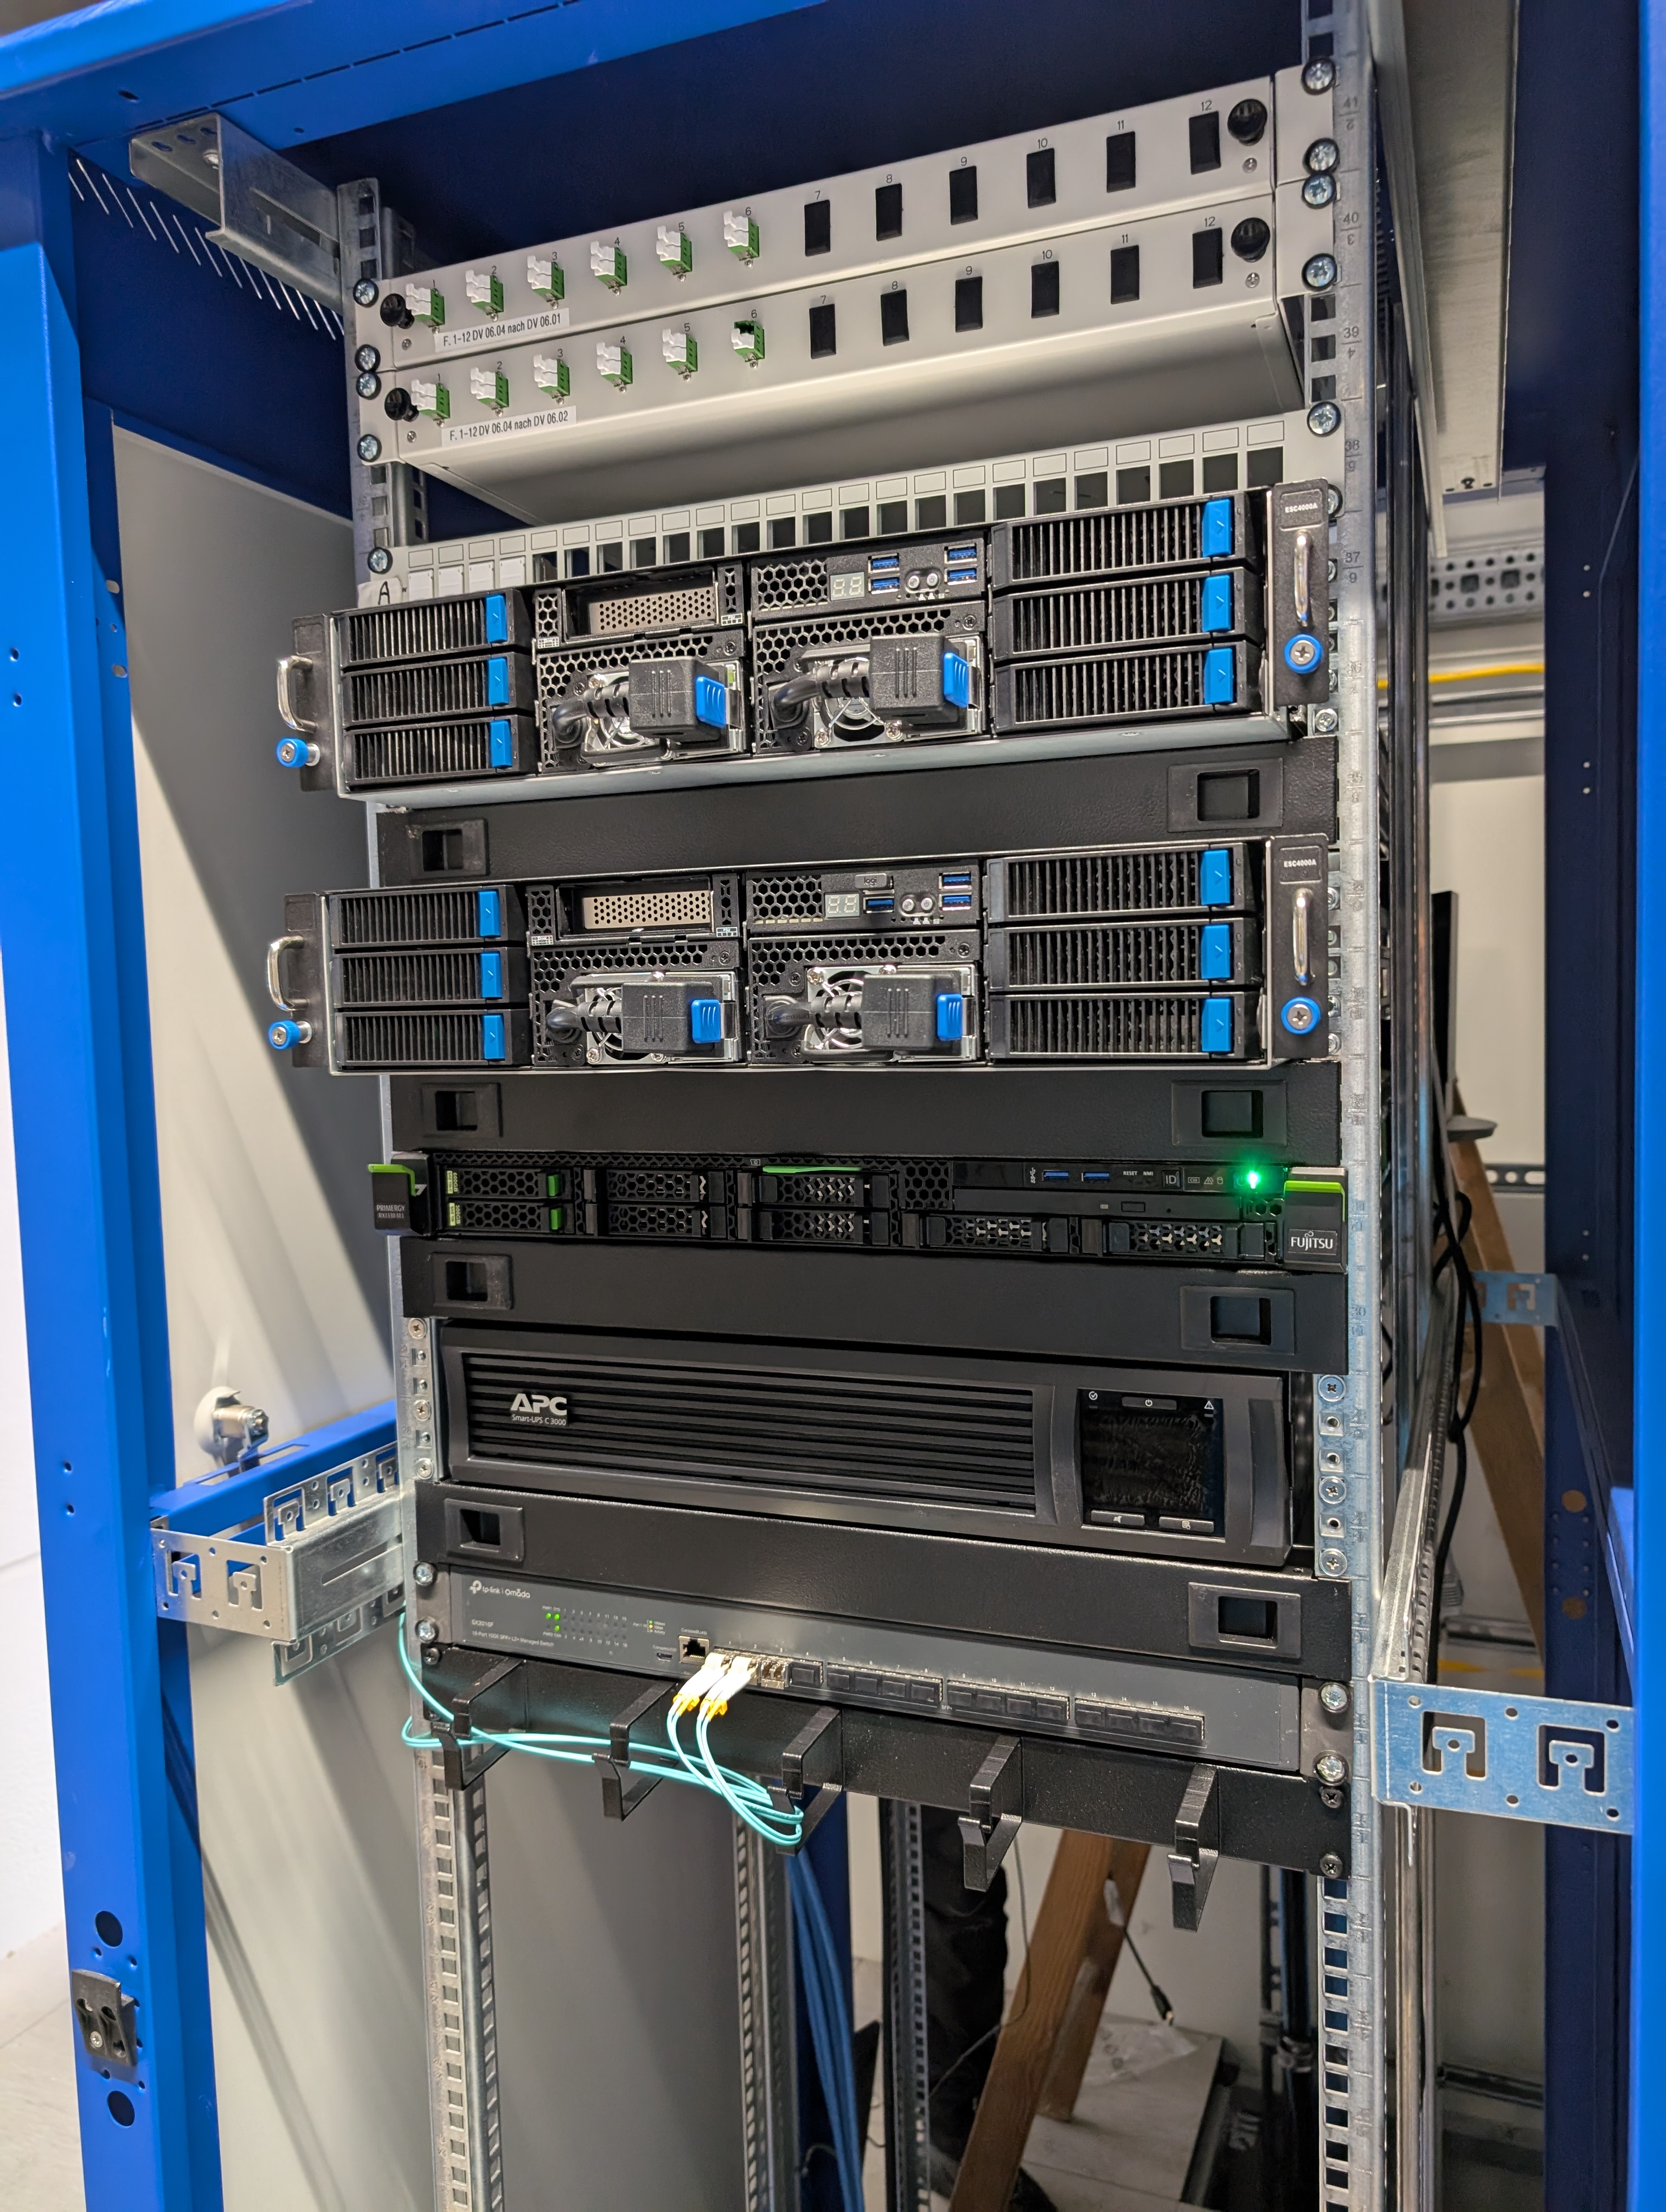
\includegraphics[width=0.95\linewidth]{imagenes/PXL_20250513_075406997.jpg}
        \captionof{figure}{}
        \label{fig:detalle-instalacion2}
    \end{center}

    \newpage
    \section{Conexión Remota y Acceso al Servidor}

    La operación del servidor, ubicado en la Universidad de Granada (España), se realiza de forma remota desde Darmstadt (Alemania), donde se llevan a cabo las prácticas extracurriculares en la empresa Desion. Esto exige una conexión remota eficiente para el desarrollo del TFG.

    Es crucial reconocer que el acceso remoto es un punto crítico de seguridad en cualquier infraestructura. Por ello, siempre se recomienda aplicar principios como la restricción de privilegios, la trazabilidad mediante auditorías y la automatización dentro de lo posible. Esto minimiza errores humanos y aumenta la resiliencia operativa.

Para el acceso se emplea SSH (Secure Shell), un protocolo estándar que cifra la comunicación en red. Aunque el puerto por defecto de SSH es el 22, su uso predeterminado lo convierte en un objetivo frecuente de ataques automatizados, como los de fuerza bruta. Utilizar puertos no estándar, como el usado en el servidor principal, en este caso, reduce la exposición directa a estos escaneos y aumenta la seguridad.

Aunque se intentó una conexión directa vía VPN, problemas de configuración en el servidor principal impidieron esta opción. Por ello, se optó por una alternativa que requiere dos saltos de conexión: el primero a una máquina intermedia (máquina-A) y el segundo al servidor objetivo (máquina-B). Por motivos de seguridad, y para proteger información sensible, los nombres de host y usuarios específicos se omiten en esta documentación. La metodología de conexión se detalla a continuación.

\subsubsection*{Pasos para la Conexión Remota}

\noindent\textbf{1. Conexión a la Máquina Intermediaria (Máquina A)}\\
La conexión se establece primero con una máquina intermedia de la Universidad de Granada. Este paso es necesario debido a la imposibilidad de una conexión VPN directa con el servidor principal.

\begin{center}
\begin{minipage}{0.95\linewidth}
\begin{verbatim}
ssh user@maquina-a
\end{verbatim}
\end{minipage}
\end{center}


\noindent\textbf{2. Conexión a la Máquina de Trabajo (Máquina B)}\\
Desde la máquina intermedia, se accede al servidor HPC. Se utiliza el mismo usuario que en el paso anterior. En este caso se ha abierto un puerto en específico para entrar al servidor.

\begin{center}
\begin{minipage}{0.95\linewidth}
\begin{verbatim}
ssh maquina-b -p XXXXX -vvv
\end{verbatim}
\end{minipage}
\end{center}

\noindent\textbf{Puerto -p:} Se especifica un puerto no estándar por motivos de seguridad..\\
\textbf{Opciones -vvv:} \texttt{-vvv} La opción -vvv muestra información detallada de la conexión, lo cual fue crucial para depurar problemas. Se utilizó principalmente al intentar conectar directamente con la VPN de la universidad activa, lo que permitió identificar que la VPN no estaba realizando el tunneling correctamente porque el servidor no estaba configurado para ello.

\subsubsection*{Configuración de Autenticación por Clave SSH}

Para simplificar y asegurar el acceso, se automatiza el proceso mediante autenticación por clave SSH en lugar de contraseñas, lo que evita la necesidad de introducir credenciales múltiples veces. Este método se aprendió y aplicó durante las prácticas en Alemania. La autenticación por clave mejora significativamente la seguridad al eliminar el riesgo de ataques de fuerza bruta basados en contraseñas y la exposición de credenciales, además de automatizar el acceso. Este procedimiento se realiza con la autorización del tutor.

\vspace{\baselineskip}

\noindent\textbf{1. Generar una Clave SSH}

Se genera un par de claves SSH en la máquina local. Se recomienda el algoritmo ed25519 por su seguridad y eficiencia. Ed25519 es un algoritmo de criptografía de curva elíptica relativamente moderno que se ha vuelto muy recomendado y cada vez más utilizado para claves SSH. 

\begin{center}
\begin{minipage}{0.95\linewidth}
\begin{verbatim}
ssh-keygen -t ed25519 \
-C "correo-usuario"
\end{verbatim}
\end{minipage}
\end{center}

\noindent \textbf{Tipo de Clave:} \texttt{ed25519} (algoritmo moderno y seguro).\\
\textbf{Comentario:} Se utiliza un correo electrónico para identificar la clave.\\
Passphrase: Puede dejarse vacía si no se requiere una capa adicional de seguridad.\\

\noindent La clave pública se guarda en \texttt{\~{}/.ssh/id\_ed25519.pub} y la privada en \texttt{\~{}/.ssh/id\_ed25519}.

\vspace{\baselineskip}

\noindent\textbf{2. Copiar la Clave Pública a la Máquina A}

La clave pública se copia a la máquina intermedia para establecer la confianza. Se emplea ssh-copy-id para una transferencia rápida y segura.

\begin{center}
\begin{minipage}{0.95\linewidth}
\begin{verbatim}
ssh-copy-id user@maquina-a
\end{verbatim}
\end{minipage}
\end{center}

\columnbreak

\noindent\textbf{3. Copiar la clave Pública a la Máquina B}

A continuación, la misma clave pública se copia al servidor HPC (máquina B).

\begin{center}
\begin{minipage}{0.95\linewidth}
\small
\begin{verbatim}
echo "ssh-ed25519 mi-clave" | \
ssh -p XXXX user@maquina-b "\
mkdir -p ~/.ssh; \
cat >> ~/.ssh/authorized_keys; \
chmod 700 ~/.ssh; \
chmod 600 ~/.ssh/authorized_keys"
\end{verbatim}
\end{minipage}
\end{center}

\noindent Contenido de la Clave: Se debe reemplazar \textbf{\texttt{[contenido\_de\_tu\_clave\_publica]}} con el texto exacto de tu archivo \texttt{\~{}/.ssh/id\_ed25519.pub}.\\
\textbf{Permisos:} El comando asegura que los directorios y archivos tengan los permisos adecuados para la seguridad de SSH.

\vspace{\baselineskip}

\noindent\textbf{4. Verificación de la Conexión}

\begin{center}
\begin{minipage}{0.95\linewidth}
\begin{verbatim}
ssh -J user@maquina-a \ 
user@maquina-b -p XXXX
\end{verbatim}
\end{minipage}
\end{center}
\textbf{Opción } \textbf{-J}: Usa la máquina A como salto intermedio para llegar a la máquina B.

\vspace{\baselineskip}

\noindent\textbf{5. Configuración del Archivo ~/.ssh/config}

Para simplificar la conexión y evitar comandos largos, se edita el archivo de configuración SSH en la máquina local (~/.ssh/config) añadiendo las siguientes entradas:

\begin{center}
\begin{minipage}{0.95\linewidth}
\begin{verbatim}
Host maquina-a
    HostName maquina-a
    User user

Host maquina-b
    HostName maquina-b
    User user
    Port XXXXX
    ProxyJump maquina-a
\end{verbatim}
\end{minipage}
\end{center}



\end{multicols*}

\begin{minipage}[t]{0.48\textwidth} 
    Con todo esto hemos logrado conectarnos a nuestro servidor con simplemente este comando:

    \begin{center}
    \begin{minipage}{0.95\linewidth}
    \begin{verbatim}
$ ssh maquina-b
    \end{verbatim}
    \end{minipage}
    \end{center}
    
    \begin{center}
       \begin{minipage}{0.95\linewidth}
       \small
       \begin{verbatim}
1 dispositivo tiene una \
actualización disponible.
Ejecute `fwupdmgr get-upgrades` \
para más información.
       
Last login: Fri Apr  4 16:43:37 \
2025 from X.X.X.X
[user@maquina-b ~]$
       \end{verbatim}
       \end{minipage}
       \end{center}
    
    Este proceso de autenticación basada en claves y configuración optimizada minimiza la intervención manual y reduce la complejidad del acceso, permitiendo centrar los esfuerzos en las tareas del proyecto.
    
    \section{Especificaciones del servidor}
    
    Tras conocer cómo conectarnos al servidor, damos paso a estudiar la infraestructura con la que trabajo, qué componentes la forman. 
    

\end{minipage}%
\hfill 
\begin{minipage}[t]{0.46\textwidth} 
    
    Instalando \texttt{neofetch} podemos ver sus especificaciones de manera sencilla, vamos a analizarla.
    
    \subsubsection*{Sistema Operativo}
    El servidor utiliza Fedora Linux 41 en su edición para servidores,    una distribución robusta y actualizada diseñada para entornos empresariales ofreciendo robustez y estabilidad. Tiene una arquitectura de \texttt{x86\_64}, compatible con procesadores de 64 bits y un rendimiento óptimo en tareas que requieren gran capacidad de cómputo. El kernel que usa es la versión \texttt{6.13.8-200.fc41.x86\_64}, reciente y con mejoras en seguridad, soporte de hardware y optimizaciones de rendimiento.

    \subsubsection*{Procesador (CPU)}
    El procesador instalado es un AMD EPYC 9334, basado en la arquitectura Zen 4 de la serie EPYC 9004. Este modelo destaca por su eficiencia energética y capacidad para procesamiento paralelo, características ideales para servidores. 

\end{minipage}

\begin{figure}[H]
    \centering
    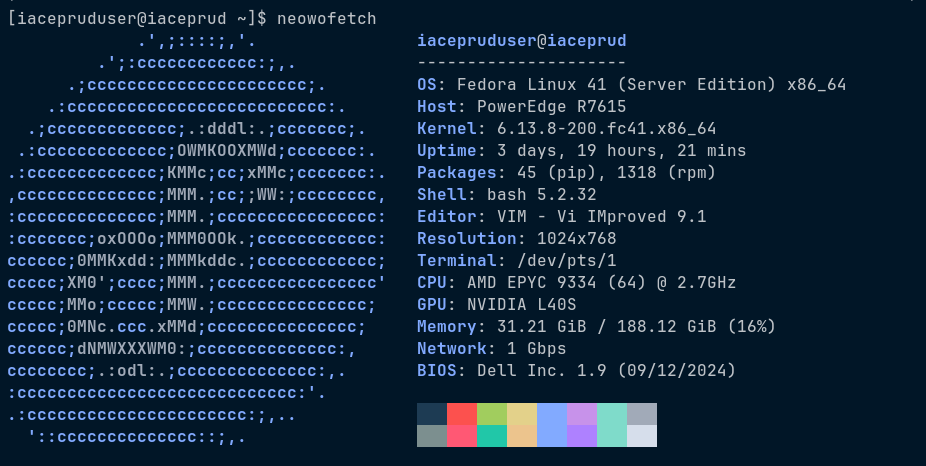
\includegraphics[width=0.8\linewidth]{imagenes/image19.png}
    \caption{Comparison of Kubernetes, Docker Swarm, Mesos and OpenShift}
    \label{fig:server2}
\end{figure}

\newpage

\begin{multicols*}{2}

Aunque el EPYC 9334 tiene 32 núcleos y 64 hilos por socket, el sistema reporta 64 núcleos físicos, lo que sugiere la presencia de dos sockets, lo que elevaría la capacidad total a 64 núcleos y probablemente 128 hilos. Esto lo convierte en una unidad excepcionalmente potente para tareas multinúcleo. Su frecuencia base es de 2.7 GHz, con capacidad para aumentar mediante turbo bajo demanda, optimizando el rendimiento en momentos de alta carga.

\subsubsection*{Memoria RAM}
Tiene 188.12 GiB de memoria RAM, utilizando tecnología DDR5 con corrección de errores (ECC), un estándar en servidores que asegura la integridad de los datos y soporta aplicaciones intensivas en memoria. Actualmente, solo el 16\% de esta capacidad está en uso, equivalente a 31.21 GiB, lo que deja un amplio margen para manejar cargas adicionales sin comprometer el rendimiento, indicando una configuración bien adaptada a las tareas actuales.


\subsubsection*{Unidad de Procesamiento Gráfico (GPU)}
El servidor está equipado con una NVIDIA L40S, una GPU de alto rendimiento diseñada para tareas avanzadas como inteligencia artificial, aprendizaje profundo, renderizado y computación científica. Esta unidad complementa la capacidad del servidor al ofrecer potencia adicional para procesamiento paralelo y aplicaciones que requieren cálculos gráficos intensivos, lo que la hace ideal para entornos que demandan un alto nivel de cómputo más allá de las capacidades de la CPU.

\subsubsection*{Red}
\begin{verbatim}
$ lspci | grep -i ethernet
\end{verbatim}

El sistema cuenta con múltiples interfaces de red Broadcom NetXtreme, incluyendo dos controladoras 10G RDMA Ethernet. Estas proporcionan alta velocidad de transmisión y baja latencia, aspectos fundamentales para mantener la disponibilidad y la fiabilidad del sistema.

Desde la perspectiva del Site Reliability Engineering, conocer en detalle estas especificaciones no es solo una cuestión informativa, sino una parte integral de la construcción de sistemas resilientes. Tal como se recomienda en las buenas prácticas de SRE, disponer de visibilidad clara sobre la infraestructura permite anticipar cuellos de botella, planificar escalabilidad y establecer mecanismos de recuperación más eficaces.

\subsection*{¿Es la infraestructura un HPC?}

La infraestructura analizada cumple con varios requisitos clave de un sistema de computación de alto rendimiento (HPC). El servidor Dell PowerEdge R7615, con Fedora Linux 41, proporciona una base robusta para cargas intensivas. Su procesador AMD EPYC 9334, con 64 núcleos y 128 hilos, junto con la GPU NVIDIA L40S orientada a IA, permite un alto paralelismo y cómputo acelerado. La RAM de 188 GiB DDR5 con ECC asegura un manejo eficiente de grandes volúmenes de datos. Aunque dispone de interfaces de red de hasta 10 Gbps, actualmente opera con una conexión de 1 Gbps, suficiente para un nodo aislado, pero limitada para un entorno HPC distribuido.

Por tanto, aunque el hardware es claramente HPC, su clasificación como sistema HPC depende del contexto operativo, no se trata de un clúster distribuido con múltiples nodos ni de una arquitectura gestionada mediante herramientas como MPI o SLURM. En su estado actual, puede considerarse un nodo de alto rendimiento preparado para tareas intensivas, pero no un sistema HPC completo.

No obstante, el uso de herramientas de orquestación como OpenShift permite desplegar servicios, simulando parcialmente el comportamiento y la gestión de cargas típico de un entorno HPC. A través de esta plataforma, es posible automatizar la asignación de recursos, escalar servicios y supervisar el rendimiento del sistema, características clave en arquitecturas distribuidas. Aunque la infraestructura se limite a un único servidor, la experiencia de operar en este entorno proporciona una aproximación práctica al modelo HPC.


\vspace{\baselineskip}

\section{Instalar los Drivers}

Se asignó la responsabilidad de instalar los controladores NVIDIA en el servidor, el cual es compartido con otros dos estudiantes. Aunque la instalación de drivers y entornos CUDA es una tarea habitual gracias a mi experiencia en prácticas, el sistema operativo actual, Fedora Linux 41, representa un contexto distinto que exige mayor precaución en comparación con distribuciones como Debian.

\vspace{\baselineskip}


\noindent\textbf{NVIDIA Optimus y su Relevancia:} 

Optimus es una tecnología de NVIDIA que integra una GPU dedicada con una GPU integrada para optimizar rendimiento y eficiencia energética. En este servidor, que incluye una GPU NVIDIA L40S junto a una GPU integrada (Matrox G200eW3), el enfoque principal es instalar los controladores que permitan aprovechar la GPU dedicada en un entorno sin interfaz gráfica.

\vspace{\baselineskip}

\noindent\textbf{Pasos para la instalación:}

\vspace{\baselineskip}

\noindent\textbf{1. Añadir los repositorios RPM Fusion}

Primero, se añaden los repositorios RPM Fusion, necesarios para obtener los paquetes de drivers no libres.

\begin{verbatim}
sudo dnf update
sudo dnf install \ 
\url{https://download1.rpmfusion.org
/free/fedora/rpmfusion-free-release-
$(rpm -E \%fedora).noarch.rpm} \url
{https://download1.rpmfusion.org/non
free/fedora/rpmfusion-nonfree-release
-$(rpm -E \%fedora).noarch.rpm}
\end{verbatim}


\noindent Se verifica:
\begin{verbatim}
sudo dnf repolist | grep \
-i rpmfusion
\end{verbatim}

\vspace{\baselineskip}

\noindent\textbf{2. Actualizar el sistema}
\begin{verbatim}
sudo dnf upgrade --refresh
\end{verbatim}

\vspace{\baselineskip}

\noindent\textbf{3. Ver qué paquetes vamos a instalar}

Ahora, en forma de tabla, detallo qué paquetes hay que instalar. Hay que tener en cuenta que es un servidor sin interfaz gráfica, por lo que podemos ahorrarnos paquetes que no vamos a usar.

\begin{itemize}
    \item \texttt{gcc}: Compilador para construir módulos
    \item \texttt{kernel-headers}: Necesario para compilar módulos del kernel
    \item \texttt{kernel-devel}: Dependencia de akmod-nvidia
    \item \texttt{akmod-nvidia}: Módulo principal de los controladores NVIDIA
    \item \texttt{xorg-x11-drv-nvidia-libs}: Librerías esenciales para CUDA
    \item \texttt{nvidia-driver}: controlador de Nvidia, para tener nvidia-smi
\end{itemize}

\vspace{\baselineskip}

\noindent\textbf{4. Comprobar el Secure Boot}

Secure Boot puede bloquear controladores no firmados, es recomendable desactivarlo.
\begin{verbatim}
mokutil --sb-state
SecureBoot disabled
\end{verbatim}

Si está desactivado, no habrá problemas; de lo contrario, consulta con el tutor o administrador para desactivarlo.
\vspace{\baselineskip}

\noindent\textbf{5. Instalación de los paquetes}
\begin{verbatim}
sudo dnf install gcc \
kernel-headers \
kernel-devel

sudo dnf install \
akmod-nvidia \
xorg-x11-drv-nvidia-libs \
nvidia-drivers
\end{verbatim}

\vspace{\baselineskip}

\noindent\textbf{6. Construcción e instalación de los módulos}
\begin{verbatim}
sudo akmods --force
sudo dracut --force
sudo reboot
\end{verbatim}

\vspace{\baselineskip}

\noindent\textbf{7. Verificación con nvidia-smi}
    
Con esto vemos que hemos instalado Nvidia Drivers 570, compatibles con la gráfica y CUDA 12.8.

\vspace{\baselineskip}

\noindent\textbf{8. Instalar Cuda Toolkit}
    
Siguiendo las instrucciones oficiales de NVIDIA para Fedora 41 descargamos el paquete de repositorio de CUDA y lo añadimos al sistema. Esto nos permitirá instalar el toolkit de CUDA, que es esencial para desarrollar aplicaciones que aprovechen la GPU.:

\begin{verbatim}
$ sudo dnf config-manager addrepo\
--from-repofile \
https://developer.download.\
nvidia.com/compute/cuda/repos\
/fedora41/x86_64/cuda-fedora41.repo

$ sudo dnf clean all
    
$ sudo dnf -y install\
 cuda-toolkit-12-8
\end{verbatim}

\noindent\textbf{9. Configurar las variables de entorno}
\begin{verbatim}
$ echo 'export PATH=/usr/local/\
cuda/bin:$PATH' >> ~/.bashrc
echo 'export LD_LIBRARY_PATH=\
/usr/local/cuda/lib64:\
$LD_LIBRARY_PATH' >> ~/.bashrc

$ source ~/.bashrc
\end{verbatim}
\vspace{\baselineskip}

\noindent\textbf{10. Verificación de la instalación}
\begin{verbatim}
$ nvcc --version
... 
Build cuda_12.8.r12.8/compiler.35583870_0
\end{verbatim}

%nvcc: NVIDIA (R) Cuda compiler driver
%Copyright (c) 2005-2025 NVIDIA Corporation
%Built on Fri_Feb_21_20:23:50_PST_2025
%Cuda compilation tools, release 12.8, V12.8.93
%Build cuda_12.8.r12.8/compiler.35583870_0

Desde la perspectiva de los principios SRE, este tipo de tarea representa mucho más que una simple instalación técnica, se trata de operar infraestructura con responsabilidad, bajo el principio de que fiabilidad y seguridad van de la mano. Con todo esto se demuestra que las acciones de personas con acceso privilegiado deben ser predecibles, auditables y reproducibles, lo cual aplica incluso en tareas aparentemente rutinarias como esta.

Ya con todo esto, tenemos un servidor con las cualidades básicas, y podemos comenzar a desplegar LLM y servicios con OpenShift.

\vspace{\baselineskip}

\section*{Problemas Encontrados}

Tras completar la instalación de los controladores NVIDIA y reiniciar el sistema con \texttt{sudo reboot}, el servidor no volvió a estar disponible. Aunque intenté depurar el fallo mediante \texttt{ssh -vvv}, no logré identificar el problema, y fue necesaria intervención directa para recuperar la conexión con el servidor. Este incidente mostró cómo incluso acciones rutinarias como un reboot pueden generar fallos críticos si no se ejecutan con las precauciones adecuadas.

También evidenció una debilidad común en entornos reales: la falta de mecanismos de visibilidad y trazabilidad inmediata ante un fallo. No contar con registros accesibles, métricas previas al apagado o algún tipo de diagnóstico automatizado complica la identificación del origen del error y ralentiza la recuperación. Esto subraya la importancia de contar con buenas prácticas de observabilidad y de preparar el entorno para análisis post-fallo.

También, durante las prácticas, un problema similar ocurrió cuando un compañero realizó una actualización en el sistema, mientras que dicho servidor tenía Secure Boot activado. Esta función de seguridad del firmware UEFI verifica que el software cargado al arrancar, como el sistema operativo y los controladores, esté firmado digitalmente por un proveedor de confianza. En este caso, al instalarse controladores no firmados, Secure Boot bloqueó el arranque, dejando el sistema inutilizable. Gracias a que el rack estaba en nuestra oficina, pude resolverlo físicamente, pero esta situación demuestra cómo una configuración mal gestionada puede dejar fuera de servicio una máquina crítica, especialmente si no se tiene acceso físico inmediato o no se ha previsto un procedimiento de recuperación.

Estos eventos refuerzan la importancia de planificar operaciones sensibles como reinicios o actualizaciones: documentarlas, validarlas en entornos previos, y prever escenarios de recuperación. En ingeniería de fiabilidad, pequeños errores operativos pueden comprometer la disponibilidad de todo el sistema, y por eso deben tratarse con el mismo rigor que los fallos de software o hardware.

\end{multicols*}

\begin{figure}[H]
    \centering
    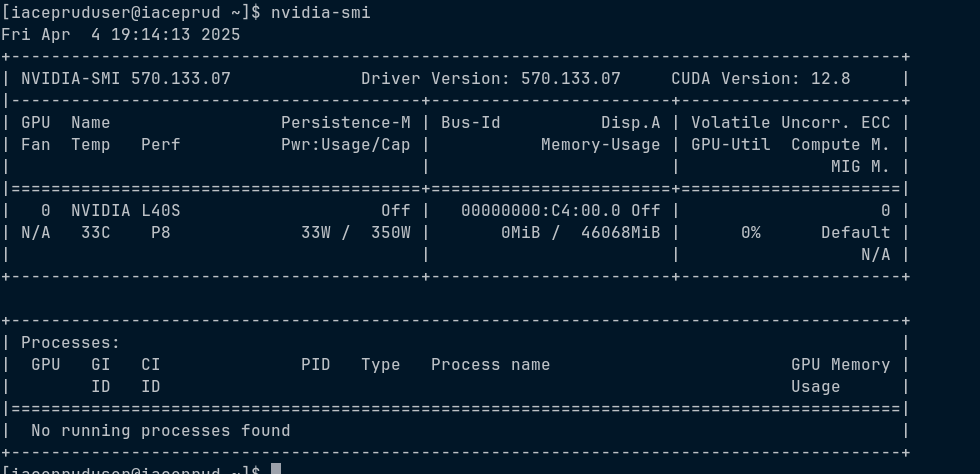
\includegraphics[width=\linewidth]{imagenes/image17.png}
    \caption{Comparison of Kubernetes, Docker Swarm, Mesos and OpenShift}
    \label{fig:server2}
\end{figure}

\newpage
\begin{multicols*}{2}


\chapter{Ejecución de LLMs en Contenedores con Podman}





\end{multicols*}

\begin{multicols*}{2}

    \chapter{Gestión Operativa con Entornos de Orquestación y Enfoque SRE}
Al desplegar una LLM (Large Language Model) con Podman, rápidamente me di cuenta de las limitaciones de una orquestación manual. Aunque Podman es excelente para la gestión de contenedores individuales, surgieron desafíos significativos al pensar en el entorno de producción. ¿Cómo podría monitorizar el rendimiento de la LLM a alto nivel, similar a lo que ofrece Grafana? Gestionar que la aplicación se adaptará a las variaciones de carga y que se mantuviera funcionando sin interrupciones se volvía una tarea compleja y propensa a errores. Además, la gestión de los logs de múltiples contenedores resultaba poco intuitiva y demandaba un esfuerzo considerable. Todas estas dificultades dejaron claro que necesitamos herramientas y estrategias que automaticen y simplifiquen estas tareas, algo fundamental para que los sistemas sean eficientes y robustos en un entorno SRE.

     En este contexto, se descubrió OpenShift, una plataforma integrada que agrupa capacidades como el escalado automático, la recuperación ante fallos, la gestión avanzada de logs y la monitorización unificada. Desde la perspectiva de SRE, OpenShift facilita la implementación de buenas prácticas desde el diseño hasta la operación, siguiendo recomendaciones sobre diseño resiliente y seguridad integrada.

     Además, la Universidad de Granada (UGR) ofreció la oportunidad de realizar un curso específico de OpenShift DO180. Aprovechando esta formación, este trabajo complementa la teoría mostrando la utilidad de OpenShift para automatizar despliegues, mejorar la observabilidad y gestionar servicios de manera eficiente.

     En este ámbito, el concepto de LLMOps es especialmente relevante. LLMOps abarca el conjunto de prácticas, herramientas y procesos para la operación eficiente de modelos de lenguaje a gran escala, incluyendo despliegue, monitorización, escalado y mantenimiento continuo en producción. Integrar prácticas de LLMOps en proyectos basados en OpenShift es un avance natural para mejorar la gestión, asegurar la escalabilidad y reducir el esfuerzo manual en la operación diaria de los modelos.


\vspace{\baselineskip}

\section{Introducción a OpenShift}

OpenShift es una plataforma que permite a las organizaciones desplegar aplicaciones en contenedores de manera eficiente y escalable. Construida sobre Kubernetes, añade una capa de abstracción y automatización que simplifica tareas esenciales del ciclo de vida de las aplicaciones, adaptándose a diversos entornos (desarrollo, pruebas, producción).

La importancia de OpenShift radica en su capacidad para gestionar aplicaciones en contenedores de forma declarativa. Los administradores definen el estado deseado de las aplicaciones (mediante archivos YAML o JSON), y la plataforma se encarga automáticamente de mantenerlo, ajustándose a cambios o imprevistos. Esta característica reduce la carga operativa, aporta consistencia y su integración con herramientas de observabilidad y flujos de trabajo de desarrollo la hace atractiva para entornos empresariales que buscan agilidad y confiabilidad.

En cuanto a su funcionamiento, OpenShift utiliza contenedores para empaquetar aplicaciones y sus dependencias, ofreciendo aislamiento respecto al sistema operativo del host. A diferencia de las máquinas virtuales, los contenedores comparten el kernel subyacente y operan en espacios aislados (namespaces), lo que disminuye la carga del sistema y mejora la portabilidad de las aplicaciones.

\begin{figure}[H]
    \centering
    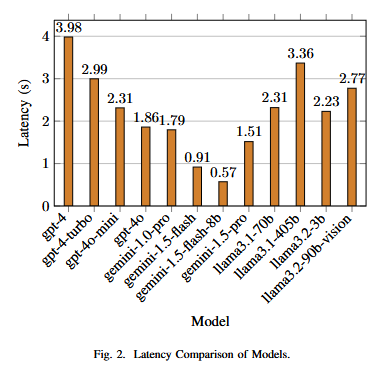
\includegraphics[width=\linewidth]{imagenes/image37.png}
    \caption{Aplicaciones en contenedores frente al sistema operativo del host}
    \label{fig:server2}
\end{figure}

\subsection{Tipos de instalación}

OpenShift ofrece varias opciones de instalación, adaptadas a las necesidades específicas de cada usuario, desde entornos de desarrollo hasta implementaciones de producción a gran escala.

\vspace{\baselineskip}

\noindent\textbf{OpenShift Local:} 
OpenShift Local permite implementar un clúster de OpenShift directamente en una computadora personal. Es ideal para pruebas, desarrollo y exploración inicial de la plataforma, proporcionando un entorno rápido y fácil de configurar. Su propósito principal es servir como espacio de familiarización y experimentación, no para entornos de producción. Esta es la opción seleccionada para este trabajo, permitiendo seguir utilizando el servidor para demostrar las capacidades de OpenShift.

\vspace{\baselineskip}

\noindent\textbf{Sandbox para desarrolladores:} 
Para quienes desean probar OpenShift sin costos iniciales, Red Hat ofrece el Sandbox para Desarrolladores. Este servicio proporciona acceso gratuito durante 30 días a un clúster de OpenShift compartido, útil para familiarizarse con la plataforma y realizar pruebas en un entorno controlado. Sin embargo, su naturaleza temporal y compartida lo hace inadecuado para implementaciones de producción.

\vspace{\baselineskip}

\noindent\textbf{Ediciones gestionadas de Red Hat OpenShift:} 
Las organizaciones que buscan soluciones de producción con menor carga operativa pueden optar por las Ediciones gestionadas de Red Hat OpenShift. Estas incluyen servicios en la nube administrados por Red Hat y proveedores asociados (ej. Red Hat OpenShift Service on AWS, Azure Red Hat OpenShift). En estas ediciones, Red Hat y el proveedor se encargan de la gestión, mantenimiento y actualizaciones del clúster, lo que reduce significativamente las responsabilidades del usuario, aunque puede implicar ciertas limitaciones (ej. menor control sobre la autenticación).


\subsection{Arquitectura y Componentes de OpenShift}

OpenShift se basa en la arquitectura modular de Kubernetes, extendiendo sus funcionalidades para ofrecer una plataforma robusta en la gestión de aplicaciones en contenedores. Esta combinación aprovecha la escalabilidad y tolerancia a fallos de Kubernetes, a la vez que introduce capacidades adicionales de automatización y control propias de OpenShift.

\begin{figure}[H]
    \centering
    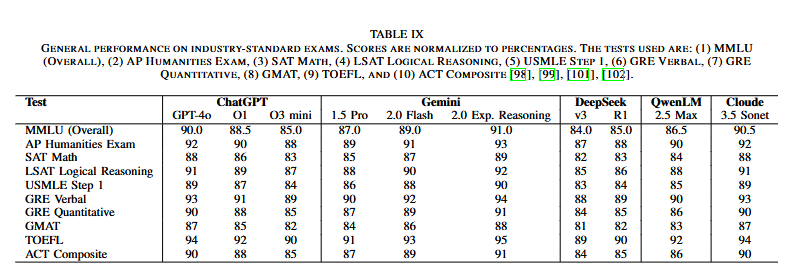
\includegraphics[width=\linewidth]{imagenes/image38.png}
    \caption{Componentes de Kubernetes}
    \label{fig:k8s-components}
\end{figure}

\subsubsection*{Componentes Fundamentales de Kubernetes}
La arquitectura de OpenShift se fundamenta en los componentes esenciales de Kubernetes. Los nodos del plano de control coordinan globalmente el clúster, gestionando la programación de cargas de trabajo y manteniendo el estado del sistema mediante servicios como la API de Kubernetes, el scheduler y el controller manager. Por su parte, los nodos del plano de cómputo ejecutan las cargas de trabajo del usuario, alojando los pods con las aplicaciones en contenedores. Esta separación mejora la estabilidad y seguridad, previniendo interferencias y reforzando la escalabilidad y tolerancia a fallos.

La API de Kubernetes, enriquecida en OpenShift con recursos personalizados, permite definir las cargas de trabajo mediante un modelo de configuración declarativa. Los usuarios especifican el estado deseado de las aplicaciones a través de archivos YAML o JSON, y OpenShift se encarga de mantenerlo automáticamente. Este enfoque sigue un ciclo de "Definir → Aplicar → Monitorizar → Ajustar", lo que reduce errores manuales y simplifica la gestión a gran escala. Además, los espacios de nombres (namespaces) son cruciales para organizar y aislar recursos dentro del clúster, facilitando la gestión granular de permisos y el control de acceso en entornos multi-equipo o multi-proyecto.

\begin{figure}[H]
    \centering
    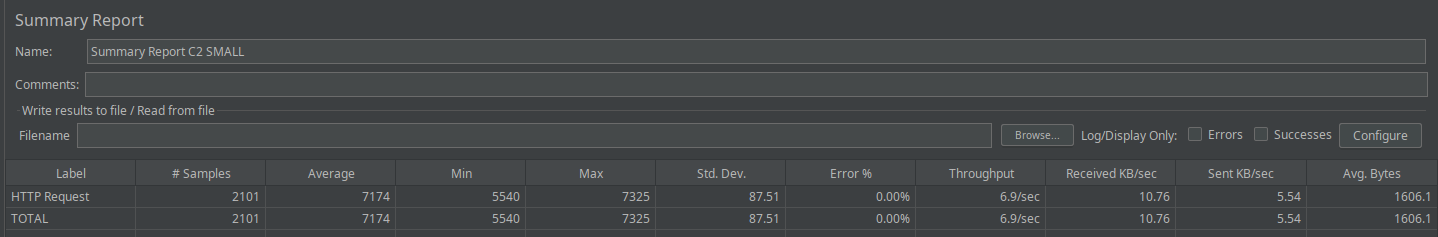
\includegraphics[width=\linewidth]{imagenes/image39.png}
    \caption{Gestión de recursos declarativa}
    \label{fig:declarative-management}
\end{figure}

\subsubsection*{Extensiones específicas de OpenShift}
OpenShift amplía las capacidades de Kubernetes con herramientas diseñadas para optimizar el flujo de trabajo de desarrollo y operaciones. Su entorno integrado para desarrolladores simplifica el ciclo de vida de las aplicaciones.

El registro de contenedores incorporado permite almacenar y gestionar imágenes de forma nativa, eliminando la necesidad de soluciones externas y mejorando la seguridad. Para automatizar procesos, OpenShift incluye pipelines de CI/CD listos para usar, que facilitan la integración y entrega continua con mínima intervención manual.

Otra herramienta poderosa es Source-to-Image (S2I), que crea imágenes de contenedores directamente desde el código fuente en repositorios como Git. Esto agiliza la construcción y estandariza las imágenes, reduciendo errores y aumentando la eficiencia del desarrollo.

En cuanto a observabilidad, OpenShift ofrece un conjunto completo de herramientas para monitorear aplicaciones e infraestructura. Los equipos pueden acceder a métricas en tiempo real, configurar alertas proactivas y analizar registros desde la consola web integrada. Esta visibilidad es crucial para mantener la confiabilidad y el rendimiento de las aplicaciones en producción, permitiendo detectar y resolver problemas de forma proactiva.

\subsection{OpenShift y SRE}

Una de las cualidades más destacadas de OpenShift es su capacidad para facilitar la implementación de prácticas SRE, al añadir un entorno robusto y flexible a Kubernetes.

\noindent\textbf{Automatización y escalabilidad:}  
OpenShift incorpora mecanismos avanzados como el autoescalado horizontal (HPA) y operadores para gestionar recursos dinámicamente. Esto permite que las aplicaciones se adapten automáticamente a fluctuaciones en la demanda sin intervención manual constante. La plataforma automatiza tareas operativas críticas como el aprovisionamiento de recursos y el balanceo de carga, reduciendo errores humanos y manteniendo la estabilidad del sistema bajo cargas variables.

\noindent\textbf{Observabilidad proactiva:}  
La plataforma integra soluciones como Prometheus para recolección de métricas y Grafana para visualización, proporcionando una visión completa y en tiempo real del estado del clúster y las aplicaciones. Esta capacidad permite monitorear el rendimiento actual y establecer alertas predictivas. Los equipos pueden detectar anomalías tempranamente, investigar incidentes mediante análisis forenses detallados y realizar mejoras continuas basadas en datos concretos.

\noindent\textbf{Gestión del ciclo de vida con CI/CD:}  
OpenShift simplifica los flujos de trabajo de integración y despliegue continuo mediante herramientas como Jenkins y Tekton. La plataforma soporta estrategias avanzadas de despliegue (ej. rolling updates, despliegues azul-verde), permitiendo implementar cambios con mínimo riesgo. En caso de problemas, los rollbacks automatizados garantizan una rápida recuperación. Todo esto facilita el equilibrio entre velocidad de entrega y estabilidad operacional.

\noindent\textbf{Resiliencia y seguridad integrada:}  
La arquitectura de OpenShift está diseñada para alta disponibilidad, con características como replicación automática de pods y distribución inteligente de cargas de trabajo. Las Security Context Constraints (SCC) implementan el principio de mínimo privilegio, mientras que el cifrado de datos en tránsito y en reposo protege la información sensible. El control de acceso granular mediante RBAC (Role-Based Access Control) asegura que solo usuarios autorizados realicen cambios críticos en el sistema.

\end{multicols*}

\begin{figure}[H]
    \centering
    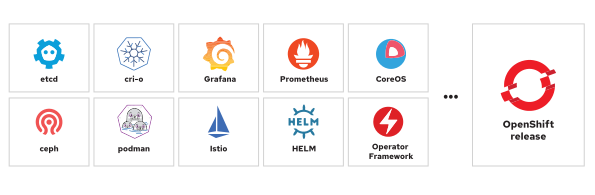
\includegraphics[width=0.85\linewidth]{imagenes/image40.png}
    \caption{Proyectos de código abierto en una versión de OpenShift}
    \label{fig:openshift-ecosystem}
\end{figure}
\noindent\textit{La integración con el ecosistema CNCF (Cloud Native Computing Foundation) asegura interoperabilidad y flexibilidad.}

\vspace{\baselineskip}
%tutorial


\section{Despliegue y administración de aplicaciones}

Esta sección detalla el proceso de despliegue y gestión de una aplicación full-stack en OpenShift. En la demostración se realiza sobre el entorno OpenShift Sandbox proporcionado por Red Hat, ya que la virtualización de OpenShift Local impidió la conexión con la GPU del servidor y las limitaciones del port forwarding (posiblemente por la gestión de dos saltos de conexión) obstaculizaron el acceso a la interfaz web. Este entorno simulará un ecosistema de producción con el fin de demostrar y validar los principios fundamentales de Site Reliability Engineering (SRE). Este enfoque permite ilustrar el uso de herramientas nativas de orquestación, aprovisionamiento, observabilidad y fiabilidad, reflejando un caso de uso realista alineado con las prácticas de Site Reliability Engineering (SRE).

Para la demostración, se utilizará la interfaz de línea de comandos (CLI) de OpenShift (\texttt{oc}), lo que garantiza la reproducibilidad de los pasos. Aunque OpenShift ofrece una potente interfaz web, todas las acciones realizadas mediante la CLI tienen su equivalente gráfico. Se utilizará para la demostración como base los tutoriales y ejemplos disponibles del repositorio \url{https://github.com/sclorg/}, que también se usan en el curso Openshift DO180 realizado.

Una recomendación a la hora de manejar la terminal es configurar alias para las cuentas de administrador y desarrollador:

\footnotesize
\begin{verbatim}
$ echo "alias al='oc login -u admin -p redhatocp https://api.ocp4.example.com:6443'"\
 >> ~/.bashrc

$ echo "alias dl='/usr/local/bin/oc login -u developer\
 -p developer https://api.ocp4.example.com:6443'" >> ~/.bashrc

$ source ~/.bashrc
\end{verbatim}

Para saber la URL de la consola web asociada a la sesión de OpenShift:
\begin{verbatim}
$ oc whoami --show-console
\end{verbatim}

Con una sesión de developer (usando el alias \texttt{dl}) es suficiente para esta demostración.

\vspace{\baselineskip}

\subsection{Source-to-Image (S2I)}

Me gustaría comenzar hablando más a fondo sobre Source-to-Image (S2I), una herramienta robusta que simplifica la creación de imágenes de contenedores reproducibles directamente desde el código fuente de una aplicación. Su propósito principal es permitir a los desarrolladores transformar su código en una imagen ejecutable de forma sencilla y eficiente, integrando el código con una imagen base ("builder image") que contiene el entorno de construcción y ejecución.

El flujo de trabajo de S2I implica la inyección del código fuente y scripts personalizados (como \texttt{assemble} y \texttt{run}) dentro de un contenedor basado en la imagen del constructor. El script \texttt{assemble} se encarga de compilar, instalar dependencias y preparar la aplicación, mientras que el script \texttt{run} la inicia. El resultado es una nueva imagen de contenedor lista para desplegar.

Generalmente, para que S2I interactúe correctamente con el código fuente, es necesario definir explícitamente scripts como \texttt{assemble}, \texttt{run}, \texttt{save-artifacts}, etc., que residen en el directorio \texttt{.s2i/bin/} del repositorio. Sin embargo, en el caso de aplicaciones Node.js estándar, como la que se encuentra en el repositorio que usamos, OpenShift sabe cómo manejar este tipo de aplicaciones internamente sin necesidad de añadir scripts personalizados al repositorio. Toma el código fuente, instala automáticamente las dependencias (\texttt{npm install}), y luego ejecuta la aplicación.

\begin{figure}[H]
    \centering
    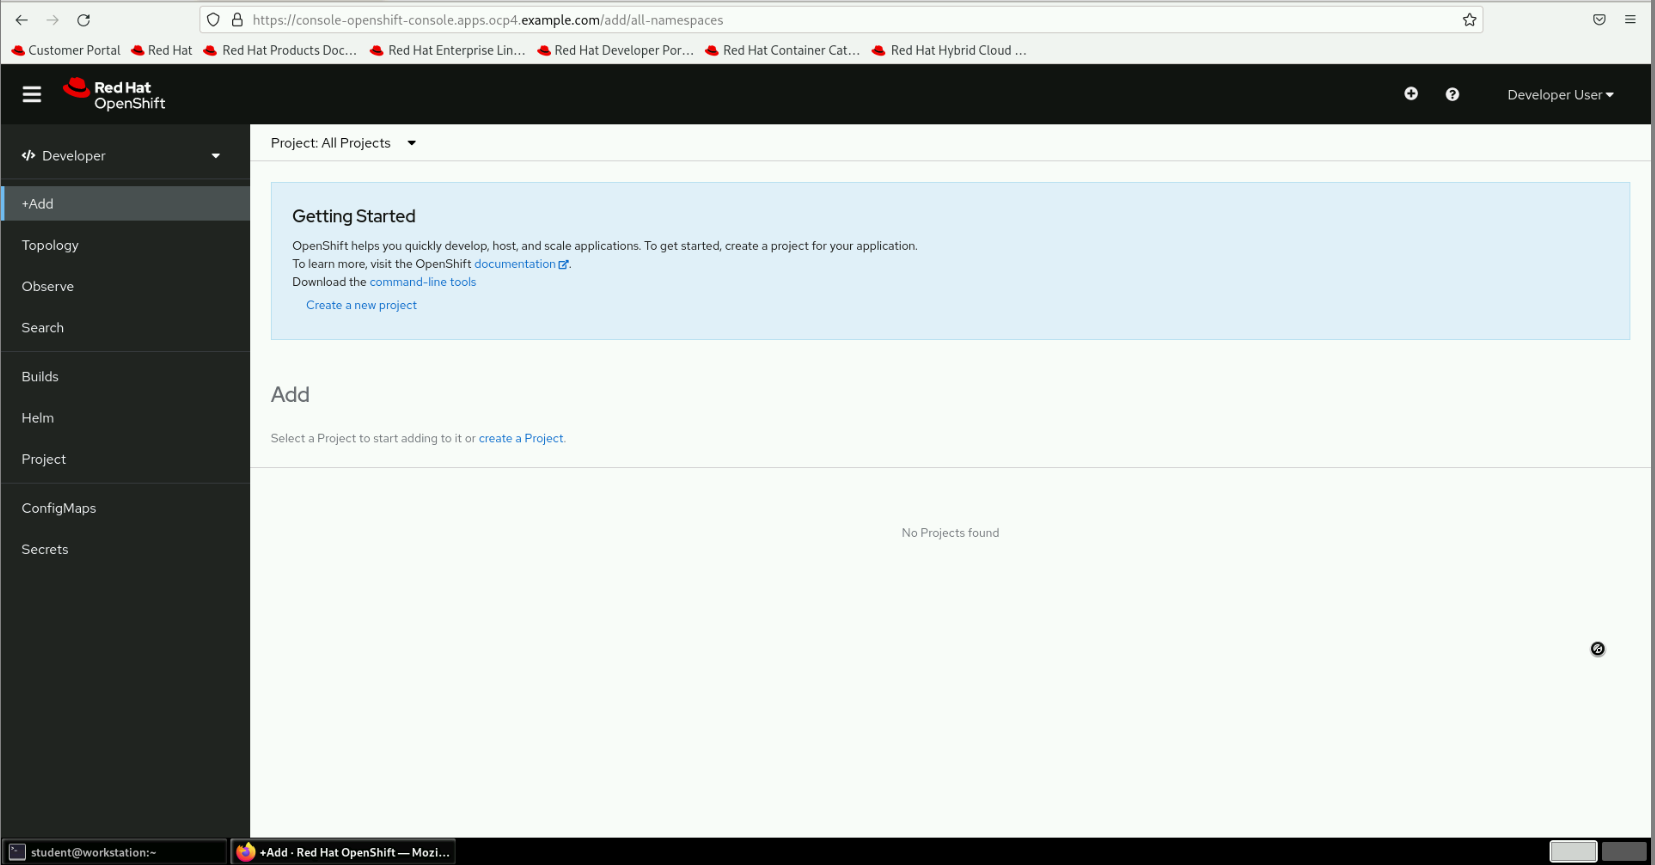
\includegraphics[width=1\linewidth]{imagenes/image4.png}
    \caption{Proceso de Source-to-Image (S2I)}
    \label{fig:openshift-ecosystem}
\end{figure}


\subsection{Creación del proyecto de trabajo}

Para aislar todos los recursos de la demostración y mantenerlos organizados, se creó un nuevo proyecto en OpenShift:
\begin{verbatim}
oc new-project sre-demo
\end{verbatim}

\subsection{Despliegue del frontend desde GitHub}

Se utilizó la aplicación de ejemplo \texttt{nodejs-ex} del repositorio de Red Hat, que contiene una interfaz web básica para la gestión de frutas. Dicho despliegue se realizó con el comando \texttt{oc new-app}, que, como se explicó previamente, utiliza la funcionalidad Source-to-Image (S2I):

\begin{verbatim}
oc new-app https://github.com/sclorg/nodejs-ex --name=nodejs-ex
\end{verbatim}

OpenShift detecta el tipo de aplicación (Node.js en este caso) y automáticamente crea y configura los objetos necesarios para su despliegue y gestión: un \texttt{BuildConfig}, un \texttt{DeploymentConfig} (o \texttt{Deployment} en versiones recientes de OpenShift) y un \texttt{Service}. En la vista de topología de la consola web, el pod aparecerá con un color naranja, indicando que se está creando o construyendo.

\begin{figure}[H]
    \centering
    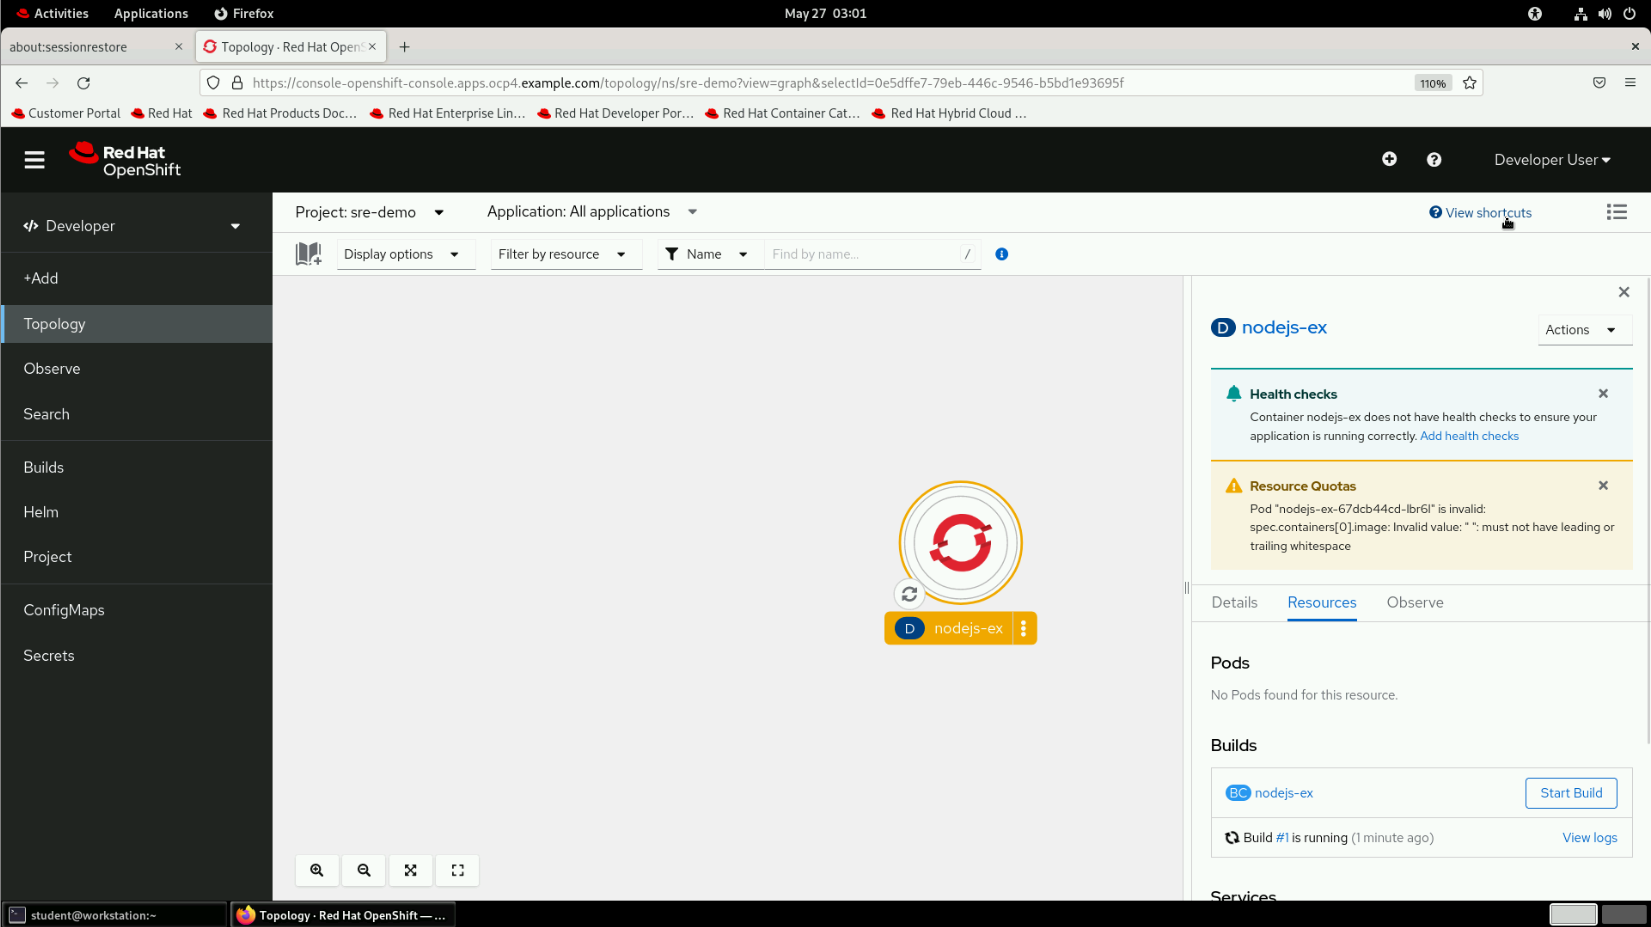
\includegraphics[width=1\linewidth]{imagenes/image11.png}
    \caption{Proceso de Source-to-Image (S2I)}
    \label{fig:openshift-ecosystem}
\end{figure}

Ahora necesitamos exponer este servicio públicamente. Con \texttt{oc expose} se genera una URL pública para acceder a la aplicación:

\begin{verbatim}
oc expose service nodejs-ex
\end{verbatim}

\begin{figure}[H]
    \centering
    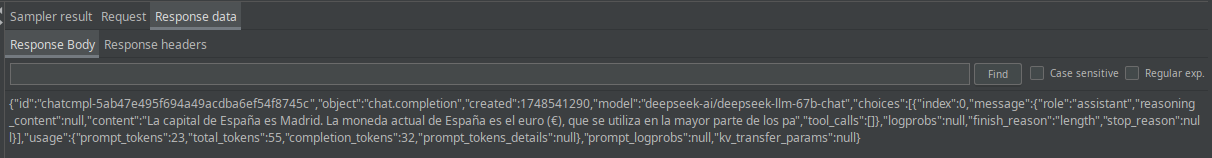
\includegraphics[width=1\linewidth]{imagenes/image9.png}
    \caption{Proceso de Source-to-Image (S2I)}
    \label{fig:openshift-ecosystem}
\end{figure}

\vspace{\baselineskip}

\subsection{Verificación y Diagnóstico del Frontend}

Al intentar interactuar con la aplicación desplegada a través de la URL generada, se desplegó la aplicación pero no podíamos realizar acciones CRUD. En principio, deberíamos ser capaces de añadir frutas a una lista, por lo que tenemos que diagnosticar el problema. Primero, se obtuvieron los pods del proyecto:
\begin{verbatim}
oc get pods
\end{verbatim}

Luego, se consultaron los logs de la instancia del pod del frontend:
\begin{verbatim}
oc logs nodejs-ex-6d6c6d6b79-ckxb8
\end{verbatim}

Los logs revelaron el siguiente error:
\begin{verbatim}
{"level":50,"time":1747902770555,"pid":21,"hostname":"nodejs-ex-6d6c6d6b79-ckxb8","err":\
{"type":"Error","message":"connect ECONNREFUSED <IP_DEL_BACKEND>:5432","stack":\
"Error: connect ECONNREFUSED <IP_DEL_BACKEND>:5432\n	at TCPConnectWrap.afterConnect \
[as oncomplete] (node:net:1607:16)","errno":-111,"code":"ECONNREFUSED","syscall":"connect"\
,"address":"<IP_DEL_BACKEND>","port":5432},"msg":"connect ECONNREFUSED <IP_DEL_BACKEND>:5432"}
\end{verbatim}

Este mensaje de \texttt{ECONNREFUSED} nos confirmó que la aplicación intenta conectarse a una base de datos PostgreSQL, que aún no estaba desplegada.




\section{Gestión de almacenamiento y configuración externa}

\subsection{Despliegue de PostgreSQL}

Para proporcionar el backend de datos, se desplegó una instancia persistente de PostgreSQL. La persistencia es crucial para que los datos de la base de datos no se pierdan si el pod se reinicia o se mueve a otro nodo. Se utilizó el siguiente comando para desplegar PostgreSQL, configurando las credenciales de usuario y la base de datos:
\begin{verbatim}
oc new-app postgresql-persistent -p POSTGRESQL_USER=user -p POSTGRESQL_PASSWORD=password\
 -p POSTGRESQL_DATABASE=nodejsdb --name=postgresql
\end{verbatim}

Este comando automatiza la creación de varios objetos clave en OpenShift: un DeploymentConfig (para gestionar el despliegue del pod de PostgreSQL), un Service denominado \texttt{postgresql} (que permite al frontend conectarse a la base de datos), un PersistentVolumeClaim (PVC) de 1Gi para la persistencia de datos, y un Secret que almacena de forma segura las credenciales.

El PersistentVolumeClaim (PVC) es una solicitud de almacenamiento por parte de la aplicación. Actúa como una abstracción que permite al pod de PostgreSQL solicitar y consumir almacenamiento persistente sin necesidad de conocer los detalles específicos de la infraestructura subyacente. OpenShift se encarga de enlazar este PVC con un PersistentVolume (un recurso de almacenamiento provisionado en el clúster) que cumpla con los requisitos del PVC, asegurando así que los datos de la base de datos no se pierdan entre reinicios o movimientos del pod. Se verifica la creación del PVC con:
\begin{verbatim}
oc get pvc
\end{verbatim}

El resultado esperado muestra el PVC en estado Bound, lo que indica la asignación exitosa de un volumen:
\begin{verbatim}
NAME        STATUS   VOLUME                              CAPACITY   ACCESS   STORAGECLASS   AGE
postgresql  Bound    pvc-8ec339dc-0fe3-4f7b-b13f-0ee6   1Gi       RWO      gp3           38s
\end{verbatim}


\begin{figure}[H]
    \centering
    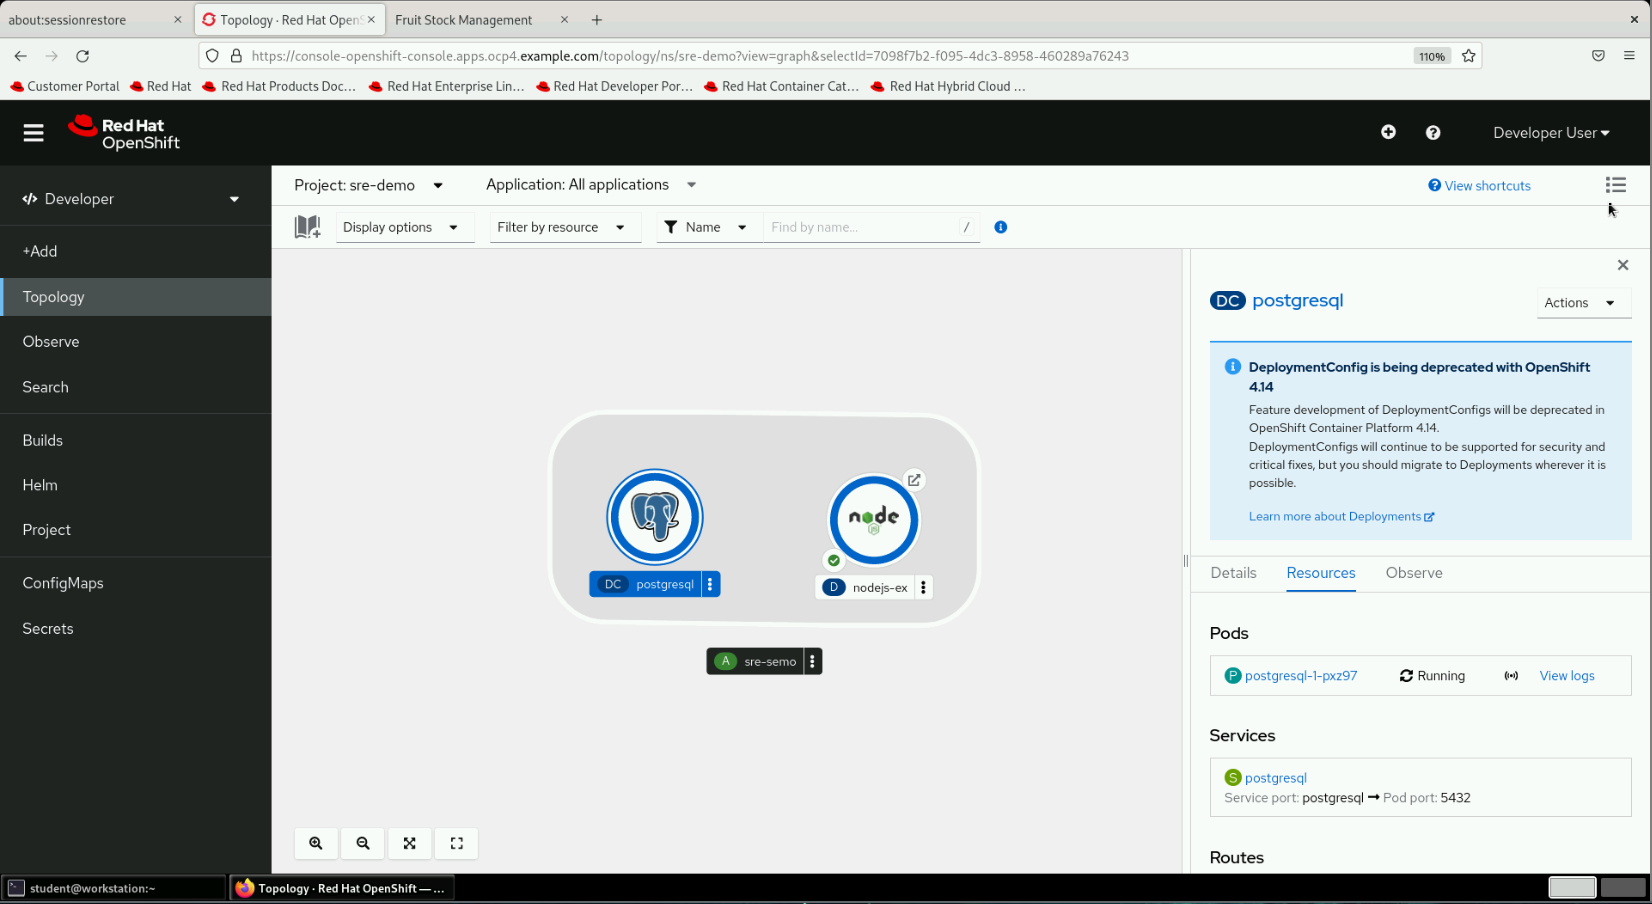
\includegraphics[width=0.95\linewidth]{imagenes/image88.png}
    \caption{Proceso de Source-to-Image (S2I)}
    \label{fig:openshift-ecosystem}
\end{figure}

Desde la interfaz web de OpenShift, se puede crear una aplicación para englobar estos pods, lo que mejora la visualización en la vista de topología. Incluso se pueden añadir etiquetas a los deployments (ej. \texttt{app.kubernetes.io/name=postgresql}, \texttt{app.kubernetes.io/name=nodejs}) para cambiar los iconos y hacerlos más visuales y organizados en la interfaz.


\subsection{Conexión del Frontend con el Backend}

Una vez que el servicio de PostgreSQL estuvo disponible y su almacenamiento configurado, se establecieron las variables de entorno en el deployment del frontend (\texttt{nodejs-ex}) para que pudiera conectarse a la base de datos recién desplegada:
\begin{verbatim}
oc set env deployment/nodejs-ex POSTGRESQL_USER=user POSTGRESQL_PASSWORD=password\
 POSTGRESQL_DATABASE=nodejsdb DATABASE_SERVICE_NAME=postgresql
\end{verbatim}

Para que el frontend aplicara estos cambios y reiniciara con las nuevas variables de entorno, se ejecutó un rollout restart:
\begin{verbatim}
oc rollout restart deployment/nodejs-ex
\end{verbatim}

Tras este paso, la aplicación del frontend comenzó a funcionar correctamente, sin el error previo de conexión a la base de datos, integrando backend con frontend. La vista de topología mostrará ahora la conexión entre el frontend y el backend.

\begin{figure}[H]
    \centering
    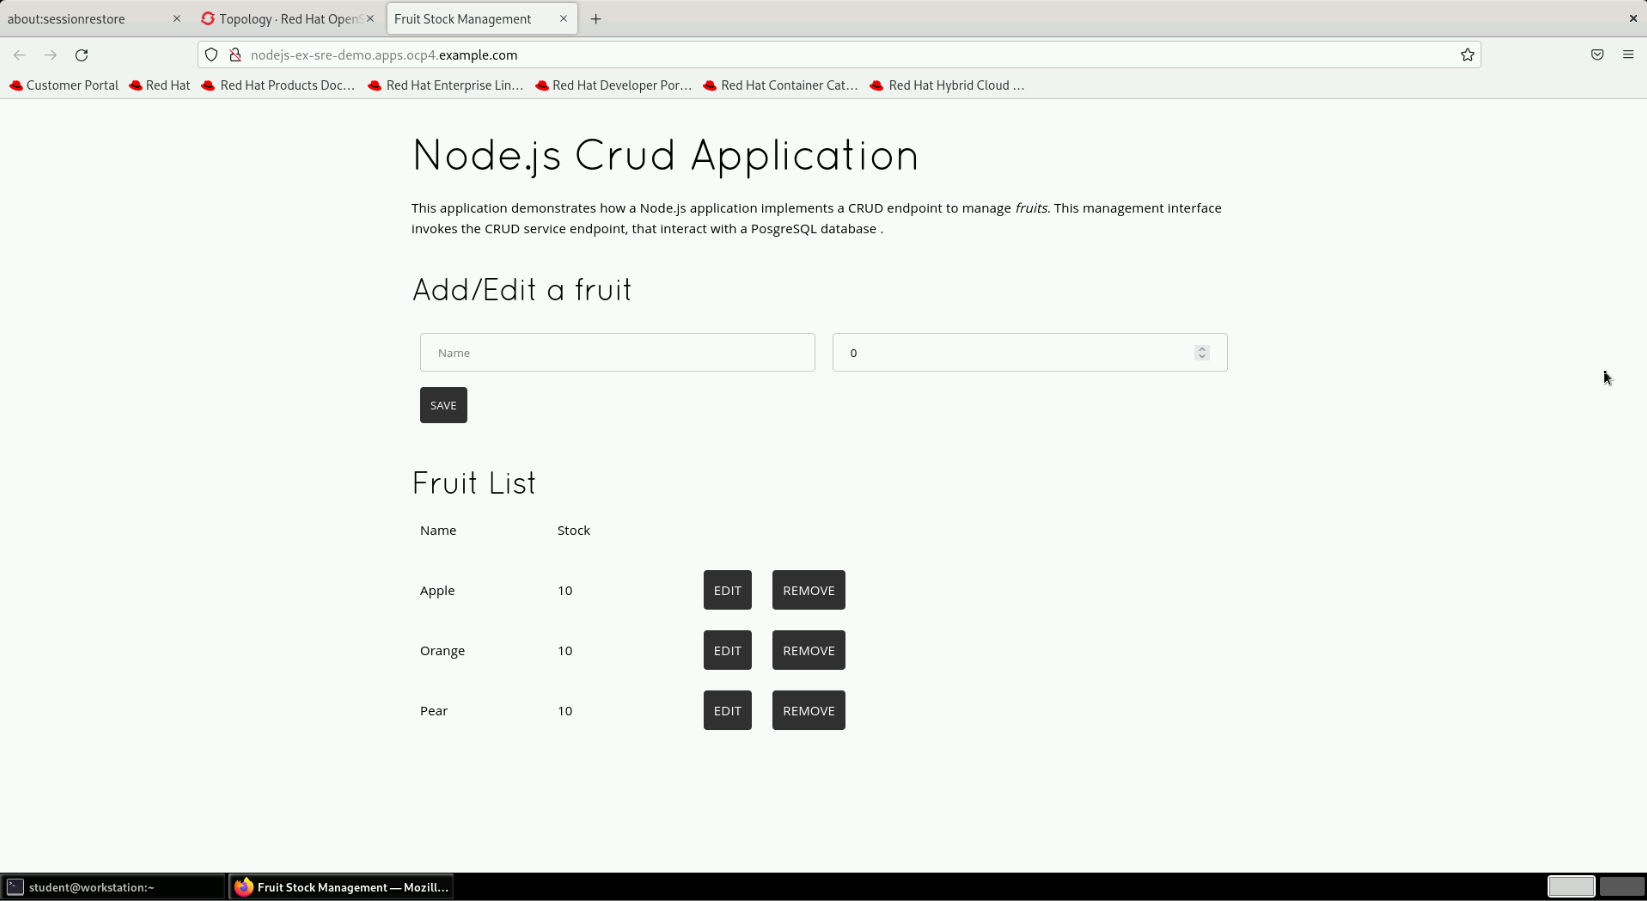
\includegraphics[width=1\linewidth]{imagenes/image12.png}
    \caption{Proceso de Source-to-Image (S2I)}
    \label{fig:openshift-ecosystem}
\end{figure}

\newpage

\section{Monitorización de cargas de trabajo}

OpenShift ofrece diversas herramientas para la monitorización, que van desde la línea de comandos hasta una consola web avanzada, importantes para la observabilidad en un entorno SRE.

\subsection{Uso de herramientas básicas desde CLI}

Para una monitorización rápida y básica del uso de recursos de pods y nodos, se emplean los siguientes comandos, que proporcionan una visión general del rendimiento del clúster:
\begin{verbatim}
oc adm top pods
oc adm top nodes
\end{verbatim}

\subsection{Monitorización avanzada (web)}

La consola web de OpenShift proporciona herramientas de observabilidad más completas, permitiendo un análisis detallado del estado de la infraestructura y las aplicaciones:

\begin{itemize}
    \item \textbf{Observe → Dashboards:} Ofrece visualizaciones gráficas de métricas clave como CPU, memoria y estado de los pods.
    \item \textbf{Observe → Metrics:} Permite realizar consultas PromQL personalizadas para un análisis al igual que Grafana.
\end{itemize}

Estas capacidades son fundamentales para establecer umbrales de alerta, configurar notificaciones proactivas y tomar decisiones informadas sobre el escalado o los ajustes de recursos.

\begin{figure}[H]
    \centering
    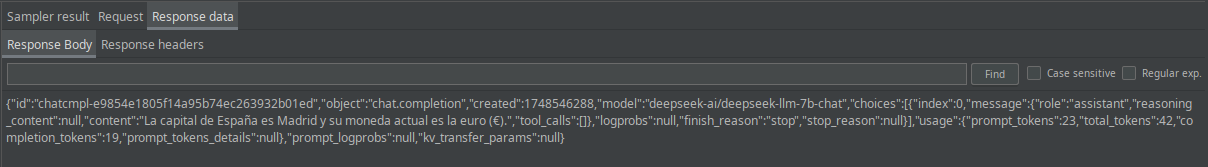
\includegraphics[width=1\linewidth]{imagenes/image20.png}
    \caption{Proceso de Source-to-Image (S2I)}
    \label{fig:openshift-ecosystem}
\end{figure}

\section{Fiabilidad, escalabilidad automática y auto-recuperación}

OpenShift incorpora características esenciales para garantizar la fiabilidad, la escalabilidad y la recuperación automática de las aplicaciones, principios fundamentales de SRE.

\subsection{Configuración de Probes (Sondas)}

Los probes (liveness y readiness) son esenciales para que OpenShift determine el estado de salud de una aplicación.  
Los probes de \textit{Liveness} le dicen a Kubernetes cuándo reiniciar un contenedor si este se ha quedado "colgado" o no responde. Esto asegura que los contenedores "muertos pero no caídos" sean reiniciados para intentar recuperarlos y mejorar la robustez de la aplicación.  
Los probes de \textit{Readiness} le dicen a Kubernetes cuándo un contenedor está listo para empezar a recibir tráfico, controlando cuándo puede recibir tráfico y garantizando que los usuarios siempre sean dirigidos a instancias que funcionan correctamente, evitando errores durante el inicio o problemas temporales.  
Ambas son evaluadas por el kubelet (agente principal que se ejecuta en cada nodo de OpenShift).

Se configuraron probes para el deployment del frontend:
\begin{verbatim}
oc set probe deployment/nodejs-ex \
  --liveness --get-url=http://:8080/ --initial-delay-seconds=15
oc set probe deployment/nodejs-ex \
  --readiness --get-url=http://:8080/ --initial-delay-seconds=5
\end{verbatim}

Con la configuración de estas sondas, el archivo YAML del deployment se habrá actualizado.


\subsection{Autoescalado}

Se habilitó el autoescalado horizontal para el deployment del frontend, de forma que OpenShift ajuste automáticamente el número de pods en función de la carga de CPU:
\begin{verbatim}
oc autoscale deployment/nodejs-ex --min=1 --max=3 --cpu-percent=50
\end{verbatim}

\begin{figure}[H]
    \centering
    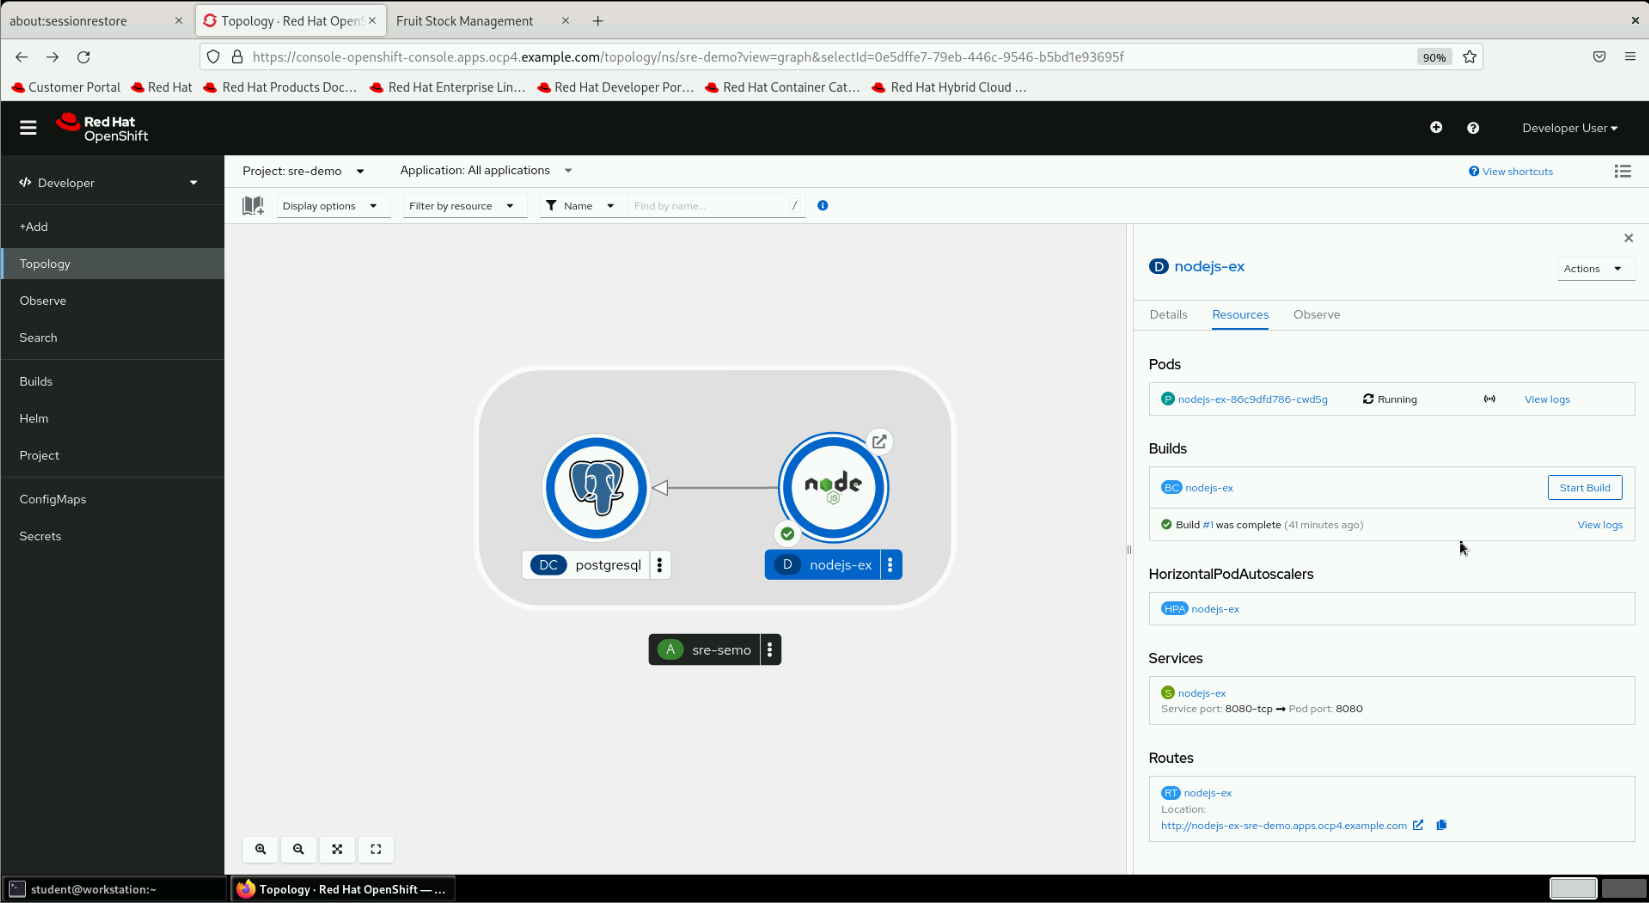
\includegraphics[width=0.8\linewidth]{imagenes/image155.png}
    \caption{Proceso de Source-to-Image (S2I)}
    \label{fig:openshift-ecosystem}
\end{figure}

Esto permite que la aplicación mantenga un rendimiento aceptable durante aumentos de demanda, sin necesidad de intervención humana.





\subsection{Recursos}

Se definieron límites y solicitudes de CPU y memoria para el deployment del frontend:
\begin{verbatim}
oc set resources deployment/nodejs-ex \
  --limits=cpu=500m,memory=512Mi \
  --requests=cpu=200m,memory=256Mi
\end{verbatim}

Esto asegura que los pods no consuman más recursos de los necesarios, y evita que un solo pod sobrecargue el nodo.

\subsection{Ejemplos prácticos de fiabilidad y recuperación}

Se llevaron a cabo una serie de pruebas para demostrar la fiabilidad inherente de OpenShift y su capacidad de auto-recuperación.

\subsubsection{Autoescalado en acción}

Para observar el comportamiento del autoescalado, se generó una carga sobre la aplicación utilizando un script que simula múltiples peticiones con ApacheBench (\texttt{ab}).  
Este es el script utilizado (\texttt{test-autoscaling.sh}):

\begin{verbatim}
#!/bin/bash

APP_URL="http://nodejs-ex-sre-demo.apps.ocp4.example.com/api/fruits"
TOTAL_REQUESTS=100000 # peticiones a enviar
CONCURRENCY=50        # peticiones simultaneas
DURATION=60           # tiempo (segundos)
echo "Iniciando ..."
echo "Duración: $DURATION segundos (puede variar)"
echo "Peticiones totales: $TOTAL_REQUESTS"
echo "Concurrencia: $CONCURRENCY"
echo "Generando carga sobre: $APP_URL"
echo "Observa con: oc get hpa -w && oc get pods -w"

# Comando ab
# -n: número de peticiones
# -c: número de peticiones concurrentes
# -t: tiempo máximo para el test (segundos) opcional podemos solo usar -n
# -k: habilita Keep-Alive HTTP (mejor rendimiento, más realista)
# -s: timeout (segundos)

ab -n $TOTAL_REQUESTS -c $CONCURRENCY -s 30 -k "$APP_URL"

echo "Test de carga con ab completado"
\end{verbatim}

Mientras la carga se generaba, se monitoreaba el estado del HPA (Horizontal Pod Autoscaler) y los pods en tiempo real para observar cómo OpenShift creaba automáticamente nuevas instancias para manejar el aumento de la demanda:
\begin{verbatim}
oc get hpa -w && oc get pods -w
\end{verbatim}

\begin{figure}[H]
    \centering
    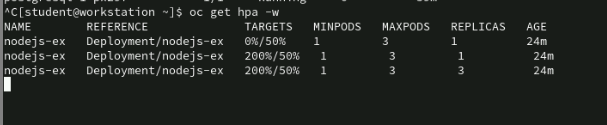
\includegraphics[width=1\linewidth]{imagenes/image27.png}
    \caption{Proceso de Source-to-Image (S2I)}
    \label{fig:openshift-ecosystem}
\end{figure}


Después de generar carga, el HPA mostró el aumento de pods hasta el máximo configurado (en este caso, 3 réplicas). ApacheBench mostró una carga significativa con \texttt{Requests per second: 2066.19 [\#/sec] (mean)} y \texttt{Time per request (mean): 24.196 [ms]}, lo que se resume en un pico de uso de CPU visible en los gráficos de monitoreo de OpenShift.

\begin{figure}[H]
    \centering
    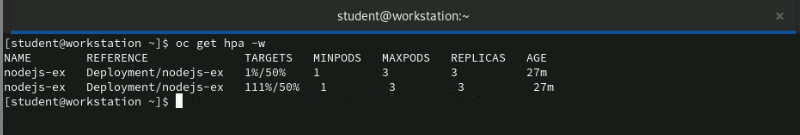
\includegraphics[width=1\linewidth]{imagenes/image7.png}
    \caption{Proceso de Source-to-Image (S2I)}
    \label{fig:openshift-ecosystem}
\end{figure}

\begin{figure}[H]
    \centering
    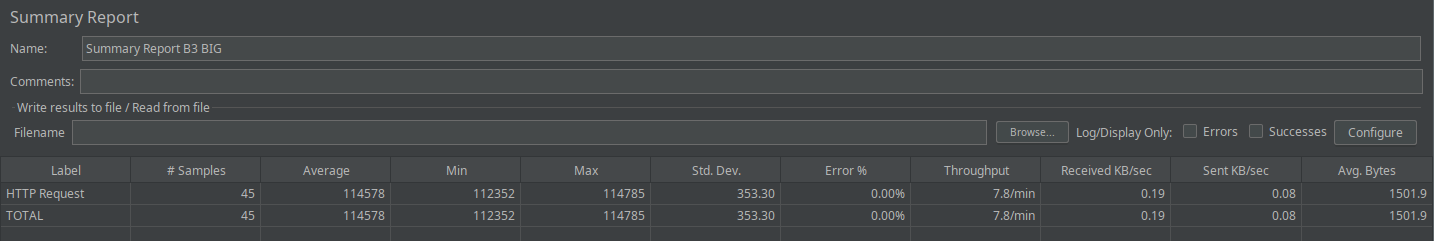
\includegraphics[width=0.95\linewidth]{imagenes/image5.png}
    \caption{Proceso de Source-to-Image (S2I)}
    \label{fig:openshift-ecosystem}
\end{figure}

\begin{figure}[H]
    \centering
    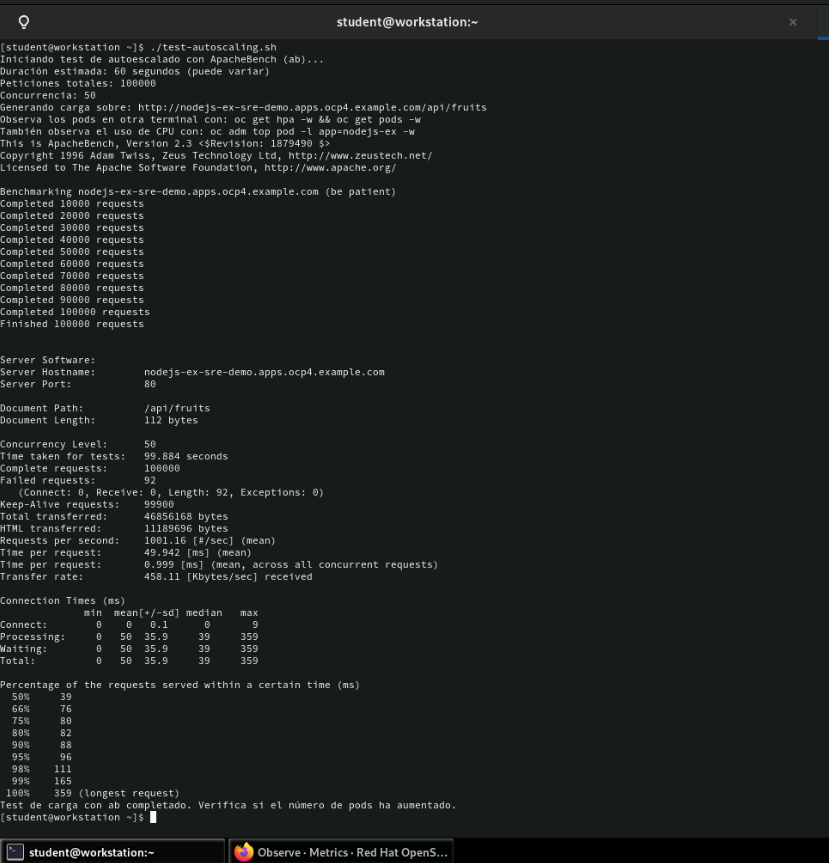
\includegraphics[width=1\linewidth]{imagenes/image144.png}
    \caption{Proceso de Source-to-Image (S2I)}
    \label{fig:openshift-ecosystem}
\end{figure}


Es importante notar que, incluso después de que la carga termine, las réplicas pueden tardar unos 5 minutos en desescalar completamente debido a la ventana de estabilización del HPA. Tras 5 minutos volverá a ser solo 1 pod.
\newpage

\begin{figure}[H]
    \centering
    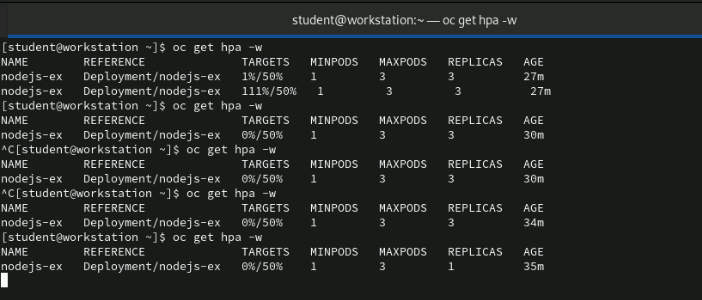
\includegraphics[width=1\linewidth]{imagenes/image1.png}
    \caption{Proceso de Source-to-Image (S2I)}
    \label{fig:openshift-ecosystem}
\end{figure}


\subsubsection{Auto-recuperación de pods}

Para demostrar la capacidad de auto-recuperación de la plataforma, se eliminó manualmente un pod de la aplicación:
\begin{verbatim}
oc delete pod $(oc get pod -l app=nodejs-ex -o name)
\end{verbatim}

OpenShift, al detectar el fallo y gracias a la configuración de sondas y réplicas, automáticamente creó un nuevo pod para reemplazar al eliminado, manteniendo así la disponibilidad del servicio sin intervención manual. Este comportamiento es posible gracias a las sondas y al deployment (siempre hay 1 como mínimo por defecto), así el sistema se recupera por sí mismo ante fallos comunes como borrar sin querer el pod.


\subsubsection{Comprobación de readiness/liveness}

Para entender cómo OpenShift reacciona a un pod que no funciona bien, se simuló un fallo en la sonda de readiness. Se cambió el puerto de la sonda de readiness a uno incorrecto (de 8080 a 9999), haciendo que la sonda falle y OpenShift marque ese pod como no listo para recibir tráfico.

Se monitorea el estado del pod en otra terminal:
\begin{verbatim}
oc get pods -w
\end{verbatim}

Luego, se ejecuta el comando para cambiar la sonda:
\begin{verbatim}
oc set probe deployment/nodejs-ex --readiness --get-url=http://:9999/ --initial-delay-seconds=5
\end{verbatim}

Tras ejecutar este comando, se observará que el pod se muestra como 0/1 Running en la columna READY. Esto significa que la sonda de readiness ha fallado para este pod, y OpenShift lo considera "no listo" para recibir tráfico.

\begin{figure}[H]
    \centering
    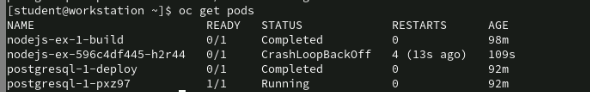
\includegraphics[width=1\linewidth]{imagenes/image16.png}
    \caption{Proceso de Source-to-Image (S2I)}
    \label{fig:openshift-ecosystem}
\end{figure}

Este resultado demuestra que la prueba de falla de readiness ha funcionado. Cuando un pod está 0/1 Ready, OpenShift lo saca del balanceador de carga. Esto significa que el tráfico se dirigirá a otros pods "listos" y, si este fuera el único pod, la aplicación sería inaccesible externamente, lo que confirma el problema inicial experimentado.

\begin{figure}[H]
    \centering
    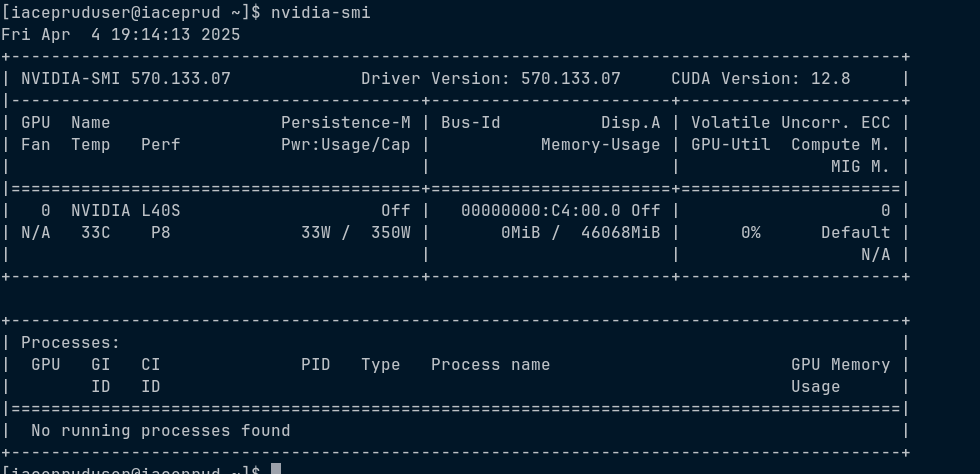
\includegraphics[width=1\linewidth]{imagenes/image6.png}
    \caption{Proceso de Source-to-Image (S2I)}
    \label{fig:openshift-ecosystem}
\end{figure}

\newpage

Posteriormente, se restauró la configuración correcta de la sonda para verificar la recuperación del estado "Ready" del pod:
\begin{verbatim}
oc set probe deployment/nodejs-ex --readiness --get-url=http://:8080/ --initial-delay-seconds=5
\end{verbatim}

\begin{figure}[H]
    \centering
    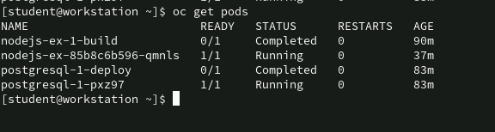
\includegraphics[width=1\linewidth]{imagenes/image177.png}
    \caption{Proceso de Source-to-Image (S2I)}
    \label{fig:openshift-ecosystem}
\end{figure}

Las sondas de Liveness se aseguran de que los contenedores "muertos pero no caídos" sean reiniciados para intentar recuperarlos, mejorando la robustez de la aplicación.  
Las sondas de Readiness controlan cuándo un contenedor puede recibir tráfico, garantizando que los usuarios siempre sean dirigidos a instancias que funcionan correctamente y evitando errores durante el inicio o problemas temporales.


\subsection{Actualización Automática de la Aplicación (CI/CD Básico)}

OpenShift facilita la implementación de un mecanismo de actualización continua cuando se realizan cambios en el repositorio de código fuente (git). Esto se logra configurando un trigger automático sobre el BuildConfig. Este comportamiento puede estar ya habilitado por defecto, pero se puede comprobar o forzar con:
\begin{verbatim}
oc set triggers bc/nodejs-ex --from-github=true --auto
\end{verbatim}

Además, en situaciones donde no se desea esperar a un push o se requiere forzar una construcción, se puede iniciar manualmente un nuevo build con el siguiente comando:
\begin{verbatim}
oc start-build nodejs-ex
\end{verbatim}

Este enfoque demuestra cómo se puede implementar un flujo básico de CI/CD (Continuous Integration/Continuous Deployment) directamente desde el control de versiones, agilizando el ciclo de entrega de software y reduciendo el esfuerzo manual.

\vspace{\baselineskip}

\newpage




\chapter{Conclusiones y Trabajos Futuros}


%\chapter{Conclusiones y Trabajos Futuros}

\nocite{*}
\printbibliography[heading=bibintoc,title={Bibliografía}]
%\bibliographystyle{miunsrturl}
%\bibliographystyle{unsrt}
%\bibliographystyle{plainnat}


%\appendix
% Aquí se incluye el manual de usuario en los apéndices
%\input{apendices/manual_usuario/manual_usuario}

% Aquí se puede incluir un paper en los apéndices
%\input{apendices/paper/paper}

% Aquí se incluye el glosario
\newglossaryentry{latex}{
  name=LaTeX,
  description={A document preparation system for high-quality typesetting}
}

\newglossaryentry{hpc}{
  name=High-Performance Computing (HPC),
  description={Área de la informática en la que el rendimiento es el principal criterio de optimización, enfocándose en la capacidad de procesar grandes volúmenes de datos y realizar cálculos complejos}
}
\addcontentsline{toc}{chapter}{Glosario}
\printglossary

\chapter*{}
\thispagestyle{empty}

\end{document}
